% Generated by Sphinx.
\def\sphinxdocclass{report}
\documentclass[a4,10pt,french]{sphinxmanual}
\usepackage[utf8]{inputenc}
\DeclareUnicodeCharacter{00A0}{\nobreakspace}
\usepackage{cmap}
\usepackage[T1]{fontenc}
\usepackage[francais]{babel}
\usepackage{times}
\usepackage[Sonny]{fncychap}
\usepackage{longtable}
\usepackage{sphinx}
\usepackage{multirow}

\addto\captionsfrench{\renewcommand{\figurename}{Fig. }}
\addto\captionsfrench{\renewcommand{\tablename}{Tableau }}
\floatname{literal-block}{Code source }



\title{Application de création de quiz}
\date{9 juin 2015}
\release{}
\author{Benoît Léo Maillard}
\newcommand{\sphinxlogo}{}
\renewcommand{\releasename}{Collège du sud, Travail de maturité}
\makeindex

\makeatletter
\def\PYG@reset{\let\PYG@it=\relax \let\PYG@bf=\relax%
    \let\PYG@ul=\relax \let\PYG@tc=\relax%
    \let\PYG@bc=\relax \let\PYG@ff=\relax}
\def\PYG@tok#1{\csname PYG@tok@#1\endcsname}
\def\PYG@toks#1+{\ifx\relax#1\empty\else%
    \PYG@tok{#1}\expandafter\PYG@toks\fi}
\def\PYG@do#1{\PYG@bc{\PYG@tc{\PYG@ul{%
    \PYG@it{\PYG@bf{\PYG@ff{#1}}}}}}}
\def\PYG#1#2{\PYG@reset\PYG@toks#1+\relax+\PYG@do{#2}}

\expandafter\def\csname PYG@tok@s2\endcsname{\def\PYG@tc##1{\textcolor[rgb]{0.25,0.44,0.63}{##1}}}
\expandafter\def\csname PYG@tok@s\endcsname{\def\PYG@tc##1{\textcolor[rgb]{0.25,0.44,0.63}{##1}}}
\expandafter\def\csname PYG@tok@nb\endcsname{\def\PYG@tc##1{\textcolor[rgb]{0.00,0.44,0.13}{##1}}}
\expandafter\def\csname PYG@tok@w\endcsname{\def\PYG@tc##1{\textcolor[rgb]{0.73,0.73,0.73}{##1}}}
\expandafter\def\csname PYG@tok@c1\endcsname{\let\PYG@it=\textit\def\PYG@tc##1{\textcolor[rgb]{0.25,0.50,0.56}{##1}}}
\expandafter\def\csname PYG@tok@kc\endcsname{\let\PYG@bf=\textbf\def\PYG@tc##1{\textcolor[rgb]{0.00,0.44,0.13}{##1}}}
\expandafter\def\csname PYG@tok@m\endcsname{\def\PYG@tc##1{\textcolor[rgb]{0.13,0.50,0.31}{##1}}}
\expandafter\def\csname PYG@tok@il\endcsname{\def\PYG@tc##1{\textcolor[rgb]{0.13,0.50,0.31}{##1}}}
\expandafter\def\csname PYG@tok@nt\endcsname{\let\PYG@bf=\textbf\def\PYG@tc##1{\textcolor[rgb]{0.02,0.16,0.45}{##1}}}
\expandafter\def\csname PYG@tok@sb\endcsname{\def\PYG@tc##1{\textcolor[rgb]{0.25,0.44,0.63}{##1}}}
\expandafter\def\csname PYG@tok@c\endcsname{\let\PYG@it=\textit\def\PYG@tc##1{\textcolor[rgb]{0.25,0.50,0.56}{##1}}}
\expandafter\def\csname PYG@tok@mh\endcsname{\def\PYG@tc##1{\textcolor[rgb]{0.13,0.50,0.31}{##1}}}
\expandafter\def\csname PYG@tok@kn\endcsname{\let\PYG@bf=\textbf\def\PYG@tc##1{\textcolor[rgb]{0.00,0.44,0.13}{##1}}}
\expandafter\def\csname PYG@tok@nc\endcsname{\let\PYG@bf=\textbf\def\PYG@tc##1{\textcolor[rgb]{0.05,0.52,0.71}{##1}}}
\expandafter\def\csname PYG@tok@gi\endcsname{\def\PYG@tc##1{\textcolor[rgb]{0.00,0.63,0.00}{##1}}}
\expandafter\def\csname PYG@tok@nn\endcsname{\let\PYG@bf=\textbf\def\PYG@tc##1{\textcolor[rgb]{0.05,0.52,0.71}{##1}}}
\expandafter\def\csname PYG@tok@nf\endcsname{\def\PYG@tc##1{\textcolor[rgb]{0.02,0.16,0.49}{##1}}}
\expandafter\def\csname PYG@tok@mb\endcsname{\def\PYG@tc##1{\textcolor[rgb]{0.13,0.50,0.31}{##1}}}
\expandafter\def\csname PYG@tok@nv\endcsname{\def\PYG@tc##1{\textcolor[rgb]{0.73,0.38,0.84}{##1}}}
\expandafter\def\csname PYG@tok@gs\endcsname{\let\PYG@bf=\textbf}
\expandafter\def\csname PYG@tok@s1\endcsname{\def\PYG@tc##1{\textcolor[rgb]{0.25,0.44,0.63}{##1}}}
\expandafter\def\csname PYG@tok@vc\endcsname{\def\PYG@tc##1{\textcolor[rgb]{0.73,0.38,0.84}{##1}}}
\expandafter\def\csname PYG@tok@si\endcsname{\let\PYG@it=\textit\def\PYG@tc##1{\textcolor[rgb]{0.44,0.63,0.82}{##1}}}
\expandafter\def\csname PYG@tok@bp\endcsname{\def\PYG@tc##1{\textcolor[rgb]{0.00,0.44,0.13}{##1}}}
\expandafter\def\csname PYG@tok@kp\endcsname{\def\PYG@tc##1{\textcolor[rgb]{0.00,0.44,0.13}{##1}}}
\expandafter\def\csname PYG@tok@gp\endcsname{\let\PYG@bf=\textbf\def\PYG@tc##1{\textcolor[rgb]{0.78,0.36,0.04}{##1}}}
\expandafter\def\csname PYG@tok@cs\endcsname{\def\PYG@tc##1{\textcolor[rgb]{0.25,0.50,0.56}{##1}}\def\PYG@bc##1{\setlength{\fboxsep}{0pt}\colorbox[rgb]{1.00,0.94,0.94}{\strut ##1}}}
\expandafter\def\csname PYG@tok@kr\endcsname{\let\PYG@bf=\textbf\def\PYG@tc##1{\textcolor[rgb]{0.00,0.44,0.13}{##1}}}
\expandafter\def\csname PYG@tok@ss\endcsname{\def\PYG@tc##1{\textcolor[rgb]{0.32,0.47,0.09}{##1}}}
\expandafter\def\csname PYG@tok@gr\endcsname{\def\PYG@tc##1{\textcolor[rgb]{1.00,0.00,0.00}{##1}}}
\expandafter\def\csname PYG@tok@se\endcsname{\let\PYG@bf=\textbf\def\PYG@tc##1{\textcolor[rgb]{0.25,0.44,0.63}{##1}}}
\expandafter\def\csname PYG@tok@sr\endcsname{\def\PYG@tc##1{\textcolor[rgb]{0.14,0.33,0.53}{##1}}}
\expandafter\def\csname PYG@tok@mf\endcsname{\def\PYG@tc##1{\textcolor[rgb]{0.13,0.50,0.31}{##1}}}
\expandafter\def\csname PYG@tok@k\endcsname{\let\PYG@bf=\textbf\def\PYG@tc##1{\textcolor[rgb]{0.00,0.44,0.13}{##1}}}
\expandafter\def\csname PYG@tok@sc\endcsname{\def\PYG@tc##1{\textcolor[rgb]{0.25,0.44,0.63}{##1}}}
\expandafter\def\csname PYG@tok@sx\endcsname{\def\PYG@tc##1{\textcolor[rgb]{0.78,0.36,0.04}{##1}}}
\expandafter\def\csname PYG@tok@vi\endcsname{\def\PYG@tc##1{\textcolor[rgb]{0.73,0.38,0.84}{##1}}}
\expandafter\def\csname PYG@tok@sd\endcsname{\let\PYG@it=\textit\def\PYG@tc##1{\textcolor[rgb]{0.25,0.44,0.63}{##1}}}
\expandafter\def\csname PYG@tok@nd\endcsname{\let\PYG@bf=\textbf\def\PYG@tc##1{\textcolor[rgb]{0.33,0.33,0.33}{##1}}}
\expandafter\def\csname PYG@tok@mi\endcsname{\def\PYG@tc##1{\textcolor[rgb]{0.13,0.50,0.31}{##1}}}
\expandafter\def\csname PYG@tok@go\endcsname{\def\PYG@tc##1{\textcolor[rgb]{0.20,0.20,0.20}{##1}}}
\expandafter\def\csname PYG@tok@cp\endcsname{\def\PYG@tc##1{\textcolor[rgb]{0.00,0.44,0.13}{##1}}}
\expandafter\def\csname PYG@tok@gh\endcsname{\let\PYG@bf=\textbf\def\PYG@tc##1{\textcolor[rgb]{0.00,0.00,0.50}{##1}}}
\expandafter\def\csname PYG@tok@sh\endcsname{\def\PYG@tc##1{\textcolor[rgb]{0.25,0.44,0.63}{##1}}}
\expandafter\def\csname PYG@tok@kt\endcsname{\def\PYG@tc##1{\textcolor[rgb]{0.56,0.13,0.00}{##1}}}
\expandafter\def\csname PYG@tok@nl\endcsname{\let\PYG@bf=\textbf\def\PYG@tc##1{\textcolor[rgb]{0.00,0.13,0.44}{##1}}}
\expandafter\def\csname PYG@tok@gd\endcsname{\def\PYG@tc##1{\textcolor[rgb]{0.63,0.00,0.00}{##1}}}
\expandafter\def\csname PYG@tok@ne\endcsname{\def\PYG@tc##1{\textcolor[rgb]{0.00,0.44,0.13}{##1}}}
\expandafter\def\csname PYG@tok@err\endcsname{\def\PYG@bc##1{\setlength{\fboxsep}{0pt}\fcolorbox[rgb]{1.00,0.00,0.00}{1,1,1}{\strut ##1}}}
\expandafter\def\csname PYG@tok@gu\endcsname{\let\PYG@bf=\textbf\def\PYG@tc##1{\textcolor[rgb]{0.50,0.00,0.50}{##1}}}
\expandafter\def\csname PYG@tok@kd\endcsname{\let\PYG@bf=\textbf\def\PYG@tc##1{\textcolor[rgb]{0.00,0.44,0.13}{##1}}}
\expandafter\def\csname PYG@tok@ge\endcsname{\let\PYG@it=\textit}
\expandafter\def\csname PYG@tok@vg\endcsname{\def\PYG@tc##1{\textcolor[rgb]{0.73,0.38,0.84}{##1}}}
\expandafter\def\csname PYG@tok@no\endcsname{\def\PYG@tc##1{\textcolor[rgb]{0.38,0.68,0.84}{##1}}}
\expandafter\def\csname PYG@tok@cm\endcsname{\let\PYG@it=\textit\def\PYG@tc##1{\textcolor[rgb]{0.25,0.50,0.56}{##1}}}
\expandafter\def\csname PYG@tok@ow\endcsname{\let\PYG@bf=\textbf\def\PYG@tc##1{\textcolor[rgb]{0.00,0.44,0.13}{##1}}}
\expandafter\def\csname PYG@tok@o\endcsname{\def\PYG@tc##1{\textcolor[rgb]{0.40,0.40,0.40}{##1}}}
\expandafter\def\csname PYG@tok@na\endcsname{\def\PYG@tc##1{\textcolor[rgb]{0.25,0.44,0.63}{##1}}}
\expandafter\def\csname PYG@tok@ni\endcsname{\let\PYG@bf=\textbf\def\PYG@tc##1{\textcolor[rgb]{0.84,0.33,0.22}{##1}}}
\expandafter\def\csname PYG@tok@gt\endcsname{\def\PYG@tc##1{\textcolor[rgb]{0.00,0.27,0.87}{##1}}}
\expandafter\def\csname PYG@tok@mo\endcsname{\def\PYG@tc##1{\textcolor[rgb]{0.13,0.50,0.31}{##1}}}

\def\PYGZbs{\char`\\}
\def\PYGZus{\char`\_}
\def\PYGZob{\char`\{}
\def\PYGZcb{\char`\}}
\def\PYGZca{\char`\^}
\def\PYGZam{\char`\&}
\def\PYGZlt{\char`\<}
\def\PYGZgt{\char`\>}
\def\PYGZsh{\char`\#}
\def\PYGZpc{\char`\%}
\def\PYGZdl{\char`\$}
\def\PYGZhy{\char`\-}
\def\PYGZsq{\char`\'}
\def\PYGZdq{\char`\"}
\def\PYGZti{\char`\~}
% for compatibility with earlier versions
\def\PYGZat{@}
\def\PYGZlb{[}
\def\PYGZrb{]}
\makeatother

\renewcommand\PYGZsq{\textquotesingle}

\begin{document}

\maketitle
\tableofcontents
\phantomsection\label{index::doc}



\chapter{Introduction}
\label{introduction:application-de-creation-de-quiz}\label{introduction::doc}\label{introduction:introduction}
Lorsqu'il nous a été demandé de choisir un séminaire pour réaliser notre travail de maturité,
ma curiosité sur tout ce qui concerne l'informatique m'a naturellement orienté
vers un projet ayant un rapport avec la programmation. Mes connaissances étaient
encore relativement faibles, ce qui n'était pas le cas de ma motivation et de ma
soif d'acquérir de nouvelles connaissances sur le sujet. La perspective de travailler
par groupe et de pouvoir partager ma passion avec d'autres personnes de mon âge rendait
ce séminaire encore plus attractif à mes yeux et j'ai donc décidé de m'y inscrire
sans trop hésiter.

Mon travail peut être divisé en deux parties distinctes, qui sont toutefois fortement
liées et qui ne pourraient pas exister indépendamment l'une de l'autre. Dans un premier
temps, il consiste au développement d'une plateforme web pédagogique permettant
la création, la résolution et la correction automatique de quiz. Cette application,
destinée à l'usage scolaire, permet à un professeur d'évaluer rapidement et de
manière ciblée le niveau de compréhension des élèves afin de pouvoir orienter
le cours en fonction du résultat obtenu. Les mathématiques sont la branche à laquelle
cette plateforme sera dédiée et un certain nombre de critères découlent donc logiquement
de cette caractéristique. Il doit être possible d'afficher des expressions mathématiques
telles que des fractions, des exposants ou des angles exprimés avec la notation adéquate.
L'application offre la possibilité aux professeurs d'analyser les résultats
obtenus par les élèves de manière globale, mais aussi de manière plus ciblée et plus
personnelle par l'intermédiaire de statistiques avancées.

En plus de cela, vu la proportion d'étudiants en possession d'un smartphone, il est
particulièrement intéressant et pratique de pouvoir utiliser le site depuis ce type
d'appareil. La partie de l'application destinée aux étudiants est parfaitement optimisée pour
les périphériques mobiles, ce qui permet une utilisation rapide dans les salles de
classe sans nécessairement avoir besoin d'un ordinateur. L'objectif final est l'intégration
de l'application au travail de groupe afin de regrouper dans un même site plusieurs outils
pédagogiques qui peuvent être utilisés de manière combinée avec les mêmes comptes d'utilisateurs.

D'autre part, le travail de développement web est accompagné
d'une documentation présentant le fonctionnement de l'application. La première partie de
cette documentation
comporte des indications à l'intention des professeurs et des étudiants pour expliquer
comment doit être utilisée l'application et faire l'inventaire de ses fonctionnalités.
Une deuxième partie plus technique accompagne ce premier chapitre, dans laquelle sont expliqués
la démarche du développement de l'application et les outils utilisés pour y parvenir. Un chapitre
un peu particulier
est consacré à RapydScript, un outil open source largement utilisé dans la réalisation
de mon projet, qui permet de générer du Javascript à partir de code Python.


\chapter{Présentation de RapydScript}
\label{rapydscript::doc}\label{rapydscript:presentation-de-rapydscript}

\section{Pourquoi utiliser Python plutôt que Javascript ?}
\label{rapydscript:pourquoi-utiliser-python-plutot-que-javascript}
Les sites web d'aujourd'hui utilisent de plus en plus le Javascript afin de rendre la navigation plus confortable pour le visiteur. Les fonctionnalités offertes par ce language permettent de concevoir une grande variété d'applications utilisables directement dans le navigateur, qui s'éxécutent côté client et qui sont donc par conséquent très accessibles au grand public. Le Javascript est donc un langage quasiment incontournable pour toute personne qui s'intéresse au développement web.

Malgré cela, ce langage n'est pas forcément facile à aborder pour un programmeur habitué à coder en Java, en Python ou dans un autre langage de programmation moderne, car son fonctionnement diffère dans un certain nombre d'aspects fondamentaux. Par exemple, le Javascript est un langage orienté objet à prototype, c'est à dire que les objets utilisés en Javascript sont des copies d'objets prototypes, et non des instances de classes comme en Python et Java. On peut également mentionner d'autres différences importantes, comme la portée des variables par défaut. Afin de palier aux difficultés que peut rencontrer un développeur qui débute dans ce langage, divers outils sont apparus pour tenter de remplacer Javascript par Python, avec pour objectif de combiner les possibilités offertes par le Javascript avec la simplicité et la clarté de Python. Ce travail a pour but de présenter et expliquer les fonctionnalités de RapydScript \footnote{
\href{http://rapydscript.pyjeon.com}{http://rapydscript.pyjeon.com}. Consulté le 20 mars 2015.
}, un outil permettant d'écrire du code très semblable à du code Python et de générer du Javascript à partir de ce code.


\section{Différentes manières d'aborder le problème : CoffeeScript, Brython et RapydScript}
\label{rapydscript:differentes-manieres-d-aborder-le-probleme-coffeescript-brython-et-rapydscript}
Un certain nombre d'outils open-source tentent de faciliter l'écriture de code Javascript et différentes approches du problème sont possibles. CoffeeScript \footnote{
\href{http://coffeescript.org}{http://coffeescript.org}. Consulté le 29 mars 2015.
} est décrit par ses auteurs comme un langage à part entière, avec sa propre syntaxe, qui ressemble parfois à Python mais est surtout inspirée de celle de Ruby, qui peut être compilé en Javascript. CoffeScript permet l'écriture d'un code source plus clair et concis, le code généré est exécuté avec les mêmes performances que du code Javascript natif, mais son utilisation nécessite l'apprentissage d'un nouveau langage, ce qui peut être un problème pour un débutant.

À l'opposé, Brython \footnote{
\href{http://www.brython.info/}{http://www.brython.info/}. Consulté le 29 mars 2015.
} propose une toute autre approche : le développeur peut écrire du code en Python qui sera exécuté par un interpréteur Python entièrement codé en Javascript intégré dans la page web. C'est certainement la solution la plus fidèle à Python, puisque la syntaxe de Brython est exactement identique à celle de Python. L'accès au DOM (Document Object Model) et l'utilisation d'Ajax se fait via l'import de modules externes. Brython est donc idéal pour quelqu'un qui ne connaît pas Javascript mais possède de bonnes bases en Python. Cependant, comme la traduction en Javascript se fait en direct, l'impact sur les performances se fait ressentir et peut poser problème pour des scripts complexes. Le script de l'interpréteur (environ 10`000 lignes) doit également être inclus dans chaque page HTML qui comporte du code Brython.

RapydScript a l'avantage de combiner les qualités des deux outils cités plus haut, en permettant d'écrire du code très similaire à du code Python standard et en le compilant en Javascript. Rapydscript est donc facile à prendre en main pour n'importe quelle personne sachant coder en Python et ne limite pas la rapidité d'exécution puisque le code qui sera exécuté est tout simplement du Javascript. Il est aussi possible d'appeler n'importe quelle fonction Javascript standard et par extension d'utiliser n'importe quelle librairie externe. Ce dernier point n'est pas négligeable puisque j'ai opté pour jQuery pour développer mon application de création de quiz en ligne. Le choix de RapydScript pour la réalisation de ce travail est apparu comme évident après avoir considéré les qualités et défauts de ces différents outils. La prise en main ainsi que la compréhension de son fonctionnement a pu se faire aisément, d'autant plus que l'absence de documentation ou de tutoriel complet sur cette technologie en français constitue une motivation supplémentaire et donne un aspect inédit à ce travail.


\section{Introduction à RapydScript}
\label{rapydscript:introduction-a-rapydscript}

\subsection{Installation}
\label{rapydscript:installation}
Il est possible d'installer RapydScript en récupérant directement la dernière version sur le dépôt Github du projet.
Pour cela, il faut exécuter les commandes suivantes dans la console :

\begin{Verbatim}[commandchars=\\\{\}]
git clone git://github.com/atsepkov/RapydScript.git
\PYG{n+nb}{cd }RapydScript
npm link .
\end{Verbatim}

RapydScript est désormais installé et peut être utilisé en ligne de commande.


\subsection{Compilation}
\label{rapydscript:compilation}
Pour compiler un fichier \textbf{source.pyj} situé dans le répertoire courant, il suffit d'utiliser la commande suivante dans la console :

\begin{Verbatim}[commandchars=\\\{\}]
rapydscript source.pyj \PYGZhy{}o result.js
\end{Verbatim}

L'option \code{-o} indique à Rapydscript le chemin d'accès du fichier compilé. On peut exécuter la compilation avec d'autres options, comme l'option \code{-p}, qui produira du code Javascript indenté avec des retours à la ligne. Le code ainsi obtenu sera beaucoup plus lisible mais aussi plus volumineux.

Une liste plus exhaustive des options de compilation est disponible sur
\href{http://rapydscript.pyjeon.com/\#header-tag-doc3}{la documentation officielle de RapydScript} \footnotemark[6]

\begin{notice}{note}{Note:}
L'extension habituellement utilisée pour les fichiers RapydScript est l'extension
\code{.pyj}. Il est cependant tout à fait possible d'utiliser l'extension habituelle des fichiers Python \code{.py} ou toute autre          extension au goût de l'utilisateur.
\end{notice}


\subsection{Programmer avec RapydScript}
\label{rapydscript:programmer-avec-rapydscript}

\subsubsection{Notions de base}
\label{rapydscript:notions-de-base}
Pour un habitué de Python, la prise en main de RapydScript peut se faire très rapidement : il suffit d'écrire son programme comme si on écrivait un programme Python, même si dans certains cas particuliers il n'est pas possible de faire exactement la même chose avec RapydScript.

Pour commencer avec un exemple simple, voici en Python une fonction qui prend deux nombres en argument et retourne le plus grand. La fonction est ensuite appelée. Ce code est parfaitement valide en Python :

\begin{Verbatim}[commandchars=\\\{\}]
\PYG{k}{def} \PYG{n+nf}{maximum}\PYG{p}{(}\PYG{n}{n1}\PYG{p}{,} \PYG{n}{n2}\PYG{p}{)}\PYG{p}{:}
    \PYG{k}{if} \PYG{n}{n1} \PYG{o}{\PYGZgt{}}\PYG{o}{=} \PYG{n}{n2}\PYG{p}{:}
        \PYG{k}{return} \PYG{n}{n1}
    \PYG{k}{elif} \PYG{n}{n2} \PYG{o}{\PYGZgt{}} \PYG{n}{n1}\PYG{p}{:}
        \PYG{k}{return} \PYG{n}{n2}

\PYG{n}{maximum}\PYG{p}{(}\PYG{n}{n1}\PYG{p}{,} \PYG{n}{n2}\PYG{p}{)} \PYG{c}{\PYGZsh{}Appel de la fonction}
\end{Verbatim}

Une fois la compilation effectuée avec RapydScript, on obtient ce résultat :

\begin{Verbatim}[commandchars=\\\{\}]
\PYG{k+kd}{function} \PYG{n+nx}{maximum}\PYG{p}{(}\PYG{n+nx}{n1}\PYG{p}{,} \PYG{n+nx}{n2}\PYG{p}{)} \PYG{p}{\PYGZob{}}
    \PYG{k}{if} \PYG{p}{(}\PYG{n+nx}{n1} \PYG{o}{\PYGZgt{}=} \PYG{n+nx}{n2}\PYG{p}{)} \PYG{p}{\PYGZob{}}
        \PYG{k}{return} \PYG{n+nx}{n1}\PYG{p}{;}
    \PYG{p}{\PYGZcb{}} \PYG{k}{else} \PYG{k}{if} \PYG{p}{(}\PYG{n+nx}{n2} \PYG{o}{\PYGZgt{}} \PYG{n+nx}{n1}\PYG{p}{)} \PYG{p}{\PYGZob{}}
        \PYG{k}{return} \PYG{n+nx}{n2}\PYG{p}{;}
    \PYG{p}{\PYGZcb{}}
\PYG{p}{\PYGZcb{}}
\PYG{n+nx}{maximum}\PYG{p}{(}\PYG{l+m+mi}{5}\PYG{p}{,} \PYG{l+m+mi}{18}\PYG{p}{)}\PYG{p}{;}
\end{Verbatim}

On peut voir les opérations qu'a fait RapydScript pour traduire le code source en Javascript : Remplacer le mot clé \code{def} par \code{function}, ajouter les accolades qui englobent la fonction et les structures \code{if}, ajouter des parenthèses autour des conditions et ajouter un \code{;} à la fin de chaque instruction. On remarque aussi que les commentaires ont été supprimés, puisqu'ils sont seulement utiles dans le code source. Le code ainsi produit peut maintenant être exécuté dans n'importe quel navigateur.

Cet exemple montre cependant un cas assez peu significatif de la puissance de RapydScript puisque le code Javascript correspondant au code source est quasiment identique. Mais RapydScript permet aussi de compiler du code typique de Python, comme par exemple des boucles \code{for}, qui n'ont pas d'équivalent en Javascript.

\begin{Verbatim}[commandchars=\\\{\}]
\PYG{n}{names\PYGZus{}list} \PYG{o}{=} \PYG{p}{[}\PYG{l+s}{\PYGZdq{}}\PYG{l+s}{Paul}\PYG{l+s}{\PYGZdq{}}\PYG{p}{,} \PYG{l+s}{\PYGZdq{}}\PYG{l+s}{Marie}\PYG{l+s}{\PYGZdq{}}\PYG{p}{,} \PYG{l+s}{\PYGZdq{}}\PYG{l+s}{Pierre}\PYG{l+s}{\PYGZdq{}}\PYG{p}{,} \PYG{l+s}{\PYGZdq{}}\PYG{l+s}{Lucie}\PYG{l+s}{\PYGZdq{}}\PYG{p}{]}

\PYG{k}{for} \PYG{n}{name} \PYG{o+ow}{in} \PYG{n}{names\PYGZus{}list}\PYG{p}{:}
    \PYG{k}{print}\PYG{p}{(}\PYG{n}{name}\PYG{p}{)}
\end{Verbatim}

RapydScript produit un code équivalent en Javascript qui s'éxecutera comme en Python. Le code généré est cette fois plus complexe et des connaissances en Javascript sont nécessaires pour le comprendre. Ce type de manipulation sera étudié dans un chapitre ultérieur. On peut par exemple aussi implémenter une fonction avec des arguments qui prennent des valeurs par défaut, ce qui n'est pas possible en Javascript.


\subsubsection{Programmation orientée objet (POO)}
\label{rapydscript:programmation-orientee-objet-poo}
Ce qui fait de RapydScript un outil si puissant est principalement les possibilités qu'il offre pour faire de la Programmation orientée objet. En Javascript, la POO est basée sur le prototypage, et il est beaucoup plus complexe de créer ses propres objets, avec de l'héritage, etc. En Python, cela est beaucoup plus simple, il est donc particulièrement intéressant de pouvoir utiliser la programmation orientée objet Python pour faire de la programmation web front-end.

Encore une fois, il suffit d'écrire une classe comme on le ferait en Python:

\begin{Verbatim}[commandchars=\\\{\}]
\PYG{k}{class} \PYG{n+nc}{MyObject}\PYG{p}{:}
    \PYG{k}{def} \PYG{n+nf}{\PYGZus{}\PYGZus{}init\PYGZus{}\PYGZus{}}\PYG{p}{(}\PYG{n+nb+bp}{self}\PYG{p}{,} \PYG{n}{name}\PYG{p}{)}\PYG{p}{:}
        \PYG{n+nb+bp}{self}\PYG{o}{.}\PYG{n}{name} \PYG{o}{=} \PYG{n}{name}

    \PYG{k}{def} \PYG{n+nf}{get\PYGZus{}name}\PYG{p}{(}\PYG{n+nb+bp}{self}\PYG{p}{)}\PYG{p}{:}
        \PYG{k}{return} \PYG{n+nb+bp}{self}\PYG{o}{.}\PYG{n}{name}

\PYG{n+nb}{object} \PYG{o}{=} \PYG{n}{MyObject}\PYG{p}{(}\PYG{l+s}{\PYGZdq{}}\PYG{l+s}{Object 1}\PYG{l+s}{\PYGZdq{}}\PYG{p}{)} \PYG{c}{\PYGZsh{}Instanciation avec un paramètre}
\PYG{n+nb}{object}\PYG{o}{.}\PYG{n}{get\PYGZus{}name}\PYG{p}{(}\PYG{p}{)} \PYG{c}{\PYGZsh{}Retourne \PYGZdq{}Objet 1\PYGZdq{}}
\end{Verbatim}

Il est également possible de faire de l'héritage :

\begin{Verbatim}[commandchars=\\\{\}]
\PYG{k}{class} \PYG{n+nc}{MyObjectPlus}\PYG{p}{(}\PYG{n}{MyObject}\PYG{p}{)}\PYG{p}{:} \PYG{c}{\PYGZsh{}Classe qui hérite de la classe créée précédemment}
    \PYG{k}{def} \PYG{n+nf}{\PYGZus{}\PYGZus{}init\PYGZus{}\PYGZus{}}\PYG{p}{(}\PYG{n+nb+bp}{self}\PYG{p}{,} \PYG{n}{name}\PYG{p}{,} \PYG{n}{number}\PYG{p}{)}\PYG{p}{:}
        \PYG{n}{MyObject}\PYG{o}{.}\PYG{n}{\PYGZus{}\PYGZus{}init\PYGZus{}\PYGZus{}}\PYG{p}{(}\PYG{n+nb+bp}{self}\PYG{p}{,} \PYG{n}{name}\PYG{p}{)}
        \PYG{n+nb+bp}{self}\PYG{o}{.}\PYG{n}{number} \PYG{o}{=} \PYG{n}{number}

    \PYG{k}{def} \PYG{n+nf}{get\PYGZus{}number}\PYG{p}{(}\PYG{n+nb+bp}{self}\PYG{p}{)}\PYG{p}{:}
        \PYG{k}{return} \PYG{n+nb+bp}{self}\PYG{o}{.}\PYG{n}{number}

    \PYG{k}{def} \PYG{n+nf}{informations}\PYG{p}{(}\PYG{n+nb+bp}{self}\PYG{p}{)}\PYG{p}{:}
        \PYG{k}{return} \PYG{l+s}{\PYGZdq{}}\PYG{l+s}{Nom : }\PYG{l+s}{\PYGZdq{}} \PYG{o}{+} \PYG{n+nb+bp}{self}\PYG{o}{.}\PYG{n}{name} \PYG{o}{+} \PYG{l+s}{\PYGZdq{}}\PYG{l+s}{ /// Nombre : }\PYG{l+s}{\PYGZdq{}} \PYG{o}{+} \PYG{n+nb}{str}\PYG{p}{(}\PYG{n+nb+bp}{self}\PYG{o}{.}\PYG{n}{number}\PYG{p}{)}

\PYG{n}{objet} \PYG{o}{=} \PYG{n}{MyObjectPlus}\PYG{p}{(}\PYG{l+s}{\PYGZdq{}}\PYG{l+s}{Objet 2}\PYG{l+s}{\PYGZdq{}}\PYG{p}{,} \PYG{l+m+mi}{5}\PYG{p}{)}
\PYG{n}{objet}\PYG{o}{.}\PYG{n}{get\PYGZus{}name}\PYG{p}{(}\PYG{p}{)} \PYG{c}{\PYGZsh{}Retourne \PYGZdq{}Objet 2\PYGZdq{}}
\PYG{n}{objet}\PYG{o}{.}\PYG{n}{get\PYGZus{}number}\PYG{p}{(}\PYG{p}{)} \PYG{c}{\PYGZsh{}Retourne 5}
\PYG{n}{objet}\PYG{o}{.}\PYG{n}{informations}\PYG{p}{(}\PYG{p}{)} \PYG{c}{\PYGZsh{}Retourne \PYGZdq{}Nom : Objet 2 /// Nombre : 5\PYGZdq{}}
\end{Verbatim}

Il n'est par contre pas possible de définir des variables de classes avec RapydScript (si on définit une variable de classe, RapydScript l'ignore simplement). Cela est dû au fait qu'en Javascript, un objet n'est pas une instance d'une classe comme en Python, mais une copie d'un objet prototype. En Python, une variable de classe est en fait un attribut de l'objet \code{Class}. Il n'y a donc qu'un seul espace en mémoire pour cette variable. En Javascript, tous les attributs du prototype sont copiés à chaque fois qu'un objet est créé et il n'y a aucun équivalent aux variables de classe.


\subsubsection{Utilisation de la bibliothèque standard Python}
\label{rapydscript:utilisation-de-la-bibliotheque-standard-python}
Avec RapydScript, il est possible d'utiliser dans le code des fonctions provenant de différentes sources. La première est la bibilothèque standard de Python, c'est à dire les fonctions natives Python, telles que \code{print()}, \code{len()} ou \code{range()}.

Pour utiliser les fonctions de la bibliothèque standard Python, il faut placer l'instruction suivante au début du fichier Python :

\begin{Verbatim}[commandchars=\\\{\}]
\PYG{k+kn}{import} \PYG{n+nn}{stdlib}
\end{Verbatim}

RapydScript définira ainsi ces fonctions dans le fichier généré et leur comportement sera en quelque sorte simulé en Javascript. Ces fonctions peuvent donc être utilisées comme on le ferait en Python, dans le code source.


\subsubsection{Séparer son code en plusieurs fichiers}
\label{rapydscript:separer-son-code-en-plusieurs-fichiers}
Il est déconseillé d'écrire tout son code dans un seul fichier lorsqu'on travaille sur un gros projet. Pour séparer son code en plusieurs fichiers, RapydScript prévoit un système d'imports qui ressemble à celui de Python. Voici comment procéder pour écrire son code dans plusieurs fichiers.

Premièrement, chaque fichier du code source doit utiliser l'extension \textbf{.pyj}, qui est l'extension des fichiers RapydScript. Ensuite, ces fichiers peuvent être utilisés comme des modules et être importés depuis un autre fichier. Par exemple, si on a placé une partie du code dans un fichier \textbf{moduletest.pyj}, on ajoutera l'instruction suivante en début de fichier :

\begin{Verbatim}[commandchars=\\\{\}]
\PYG{k+kn}{import} \PYG{n+nn}{moduletest}
\end{Verbatim}

Lors de la compilation, RapydScript va rassembler tous les fichiers du code source dans un même fichier Javascript, ce qui facilite aussi l'insertion du script dans un fichier HTML. Il est important de noter, cependant, que l'import d'un module ne rend pas ses fonctions disponibles dans un espace de noms distinct. Par exemple, pour appeler la fonction \code{test()} du module de l'exemple précédent, voici comment procéder :

\begin{Verbatim}[commandchars=\\\{\}]
\PYG{k+kn}{import} \PYG{n+nn}{moduletest}

\PYG{n}{test}\PYG{p}{(}\PYG{p}{)} \PYG{c}{\PYGZsh{}Correct}
\PYG{n}{moduletest}\PYG{o}{.}\PYG{n}{test}\PYG{p}{(}\PYG{p}{)} \PYG{c}{\PYGZsh{}Ne fonctionne pas}
\end{Verbatim}


\subsubsection{Utilisation de fonctions Javascript natives ou provenant de librairies externes}
\label{rapydscript:utilisation-de-fonctions-javascript-natives-ou-provenant-de-librairies-externes}
Il est également possible d'utiliser des fonctions Javascript natives, par exemple :

\begin{Verbatim}[commandchars=\\\{\}]
\PYG{c}{\PYGZsh{}Ces deux expressions sont équivalentes :}
\PYG{n}{console}\PYG{o}{.}\PYG{n}{log}\PYG{p}{(}\PYG{l+s}{\PYGZdq{}}\PYG{l+s}{Bonjour}\PYG{l+s}{\PYGZdq{}}\PYG{p}{)} \PYG{c}{\PYGZsh{}Fonction Javascript}
\PYG{k}{print}\PYG{p}{(}\PYG{l+s}{\PYGZdq{}}\PYG{l+s}{Bonjour}\PYG{l+s}{\PYGZdq{}}\PYG{p}{)} \PYG{c}{\PYGZsh{}Fonction Python}
\end{Verbatim}

L'exemple parle de lui-même et ne nécessite pas d'explication supplémentaire. Il peut parfois être pratique d'utiliser des fonctions qui n'ont pas d'équivalent en Python.

Mais une autre grande force de RapydScript est la possibilité d'utiliser des librairies Javascript externes, telles que jQuery \footnote{
\href{https://jquery.com/}{https://jquery.com/}. Consulté le 29 mars 2015.
} ou AngularJS \footnote{
\href{https://angularjs.org/}{https://angularjs.org/}. Consulté le 29 mars 2015.
}. Pour cela, rien de plus simple, il suffit d'insérer le script de la librairie que l'on veut utiliser dans le code HTML, comme ceci :

\begin{Verbatim}[commandchars=\\\{\}]
\PYG{n+nt}{\PYGZlt{}html}\PYG{n+nt}{\PYGZgt{}}
\PYG{n+nt}{\PYGZlt{}head}\PYG{n+nt}{\PYGZgt{}}
    \PYG{n+nt}{\PYGZlt{}script }\PYG{n+na}{src=}\PYG{l+s}{\PYGZdq{}jquery.js\PYGZdq{}}\PYG{n+nt}{\PYGZgt{}}\PYG{n+nt}{\PYGZlt{}/script\PYGZgt{}}\PYG{c}{\PYGZlt{}!\PYGZhy{}\PYGZhy{}}\PYG{c}{ jQuery }\PYG{c}{\PYGZhy{}\PYGZhy{}\PYGZgt{}}
    \PYG{n+nt}{\PYGZlt{}script }\PYG{n+na}{src=}\PYG{l+s}{\PYGZdq{}myscript.js\PYGZdq{}}\PYG{n+nt}{\PYGZgt{}}\PYG{n+nt}{\PYGZlt{}/script\PYGZgt{}}\PYG{c}{\PYGZlt{}!\PYGZhy{}\PYGZhy{}}\PYG{c}{ Script créé avec RapydScript }\PYG{c}{\PYGZhy{}\PYGZhy{}\PYGZgt{}}
\PYG{n+nt}{\PYGZlt{}/head\PYGZgt{}}
\PYG{n+nt}{\PYGZlt{}body}\PYG{n+nt}{\PYGZgt{}}
    \PYG{n+nt}{\PYGZlt{}div} \PYG{n+na}{id=}\PYG{l+s}{\PYGZdq{}mydiv\PYGZdq{}}\PYG{n+nt}{\PYGZgt{}}\PYG{n+nt}{\PYGZlt{}/div\PYGZgt{}}
\PYG{n+nt}{\PYGZlt{}/body\PYGZgt{}}
\PYG{n+nt}{\PYGZlt{}/html\PYGZgt{}}
\end{Verbatim}

On peut maintenant utiliser les fonctions jQuery dans notre code. Cette fonction sélectionne le \code{\textless{}div\textgreater{}} et y insère du texte :

\begin{Verbatim}[commandchars=\\\{\}]
def add\PYGZus{}text(text):
    \PYGZdl{}(\PYGZdq{}\PYGZsh{}mydiv\PYGZdq{}).text(text)

add\PYGZus{}text(\PYGZdq{}Hello World\PYGZdq{})
\end{Verbatim}

On peut procéder de la même manière pour n'importe quelle autre librairie Javascript externe.


\chapter{Documentation utilisateur}
\label{doc-user::doc}\label{doc-user:documentation-utilisateur}

\section{Professeurs}
\label{doc-user:professeurs}

\subsection{Création de quiz}
\label{doc-user:creation-de-quiz}\begin{figure}[htbp]
\centering
\capstart

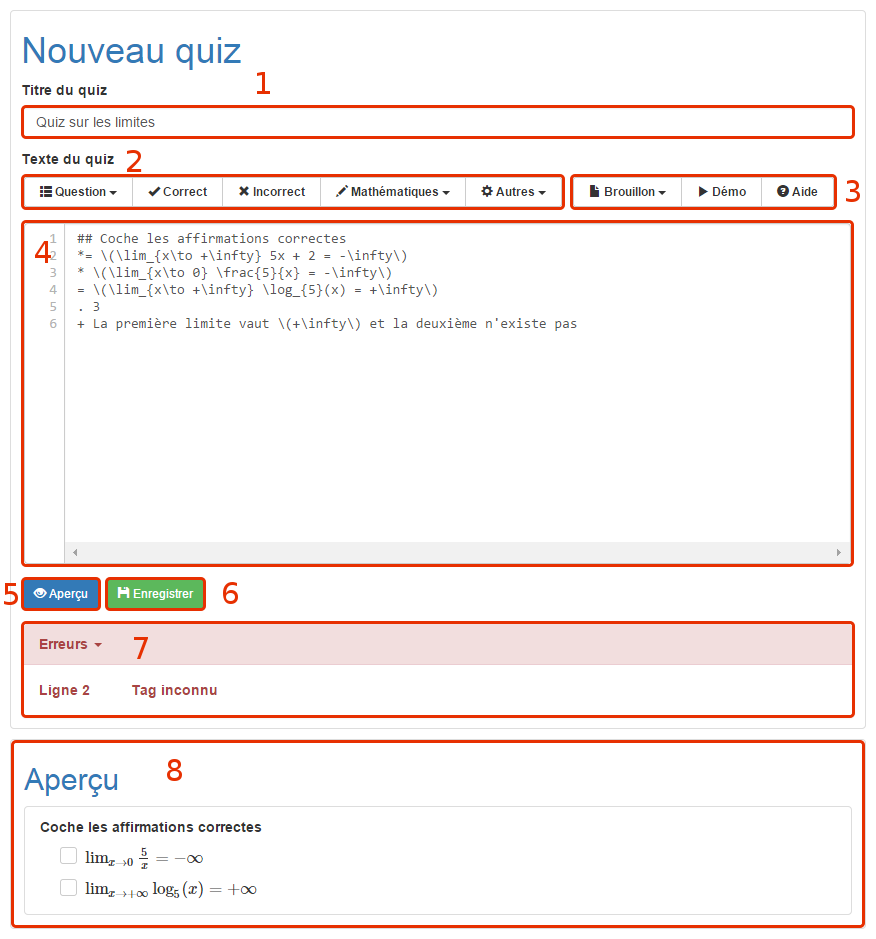
\includegraphics[width=0.700\linewidth]{create.png}
\caption{Page de création de quiz}\end{figure}


\subsubsection{Création d'une question et définition de ses caractéristiques}
\label{doc-user:creation-d-une-question-et-definition-de-ses-caracteristiques}
La création du quiz se fait par l'intermédiaire d'un langage de balisage de type Markdown pour définir les différentes questions du quiz ainsi que leurs caractéristiques. Le code du quiz doit être écrit dans la zone de texte principale \textbf{(4)} La définition des questions se fait selon le schéma suivant : Une balise avec des accolades comme \code{\{++\}} permet de définir une nouvelle question. Toutes les balises avec des accolades doivent se situer en début de ligne. Le texte de la question peut être écrit sur plusieurs lignes, chaque retour à la ligne simple est considéré comme un espace. Ensuite, divers attributs peuvent être ajoutés aux questions. Chaque attribut est également caractérisé par une balise avec des accolades.


\paragraph{Explication des balises}
\label{doc-user:explication-des-balises}
\begin{tabulary}{\linewidth}{|L|L|}
\hline
\textsf{\relax 
Balise
} & \textsf{\relax 
Signification
}\\
\hline
\{++\}
 & 
Question à choix multiple avec plusieurs options qui peuvent être choisies
\\
\hline
\{**\}
 & 
Question à choix multiple avec une seule option qui peut être choisie
\\
\hline
\{??\}
 & 
Question avec un champ de texte à remplir
\\
\hline
\{*\}
 & 
Option invalide dans un QCM
\\
\hline
\{=\}
 & 
Option valide dans un QCM
\\
\hline
\{=\}
 & 
Réponse correcte dans une question à champ de texte
\\
\hline
\{=r\}
 & 
Réponse d'une question à champ de texte définie par une expression régulière
\\
\hline
\{.\}
 & 
Permet de définir le nombre de points sur la question (par défaut, 1)
\\
\hline
\{+\}
 & 
Ajout d'un commentaire d'explication qui sera affiché lors de la correction
\\
\hline\end{tabulary}



\paragraph{Exemple de quiz avec le système de balisage}
\label{doc-user:exemple-de-quiz-avec-le-systeme-de-balisage}
\begin{Verbatim}[commandchars=\\\{\}]
\PYGZob{}++\PYGZcb{}
Énoncé de la question à choix multiple (plusieurs cases peuvent être cochées)
\PYGZob{}*\PYGZcb{} Option 1
\PYGZob{}=\PYGZcb{} Option 2 (correcte)
\PYGZob{}=\PYGZcb{} Option 4 (correcte)
\PYGZob{}+\PYGZcb{} Commentaire affiché à la correction
\PYGZob{}.\PYGZcb{} 1.5

\PYGZob{}**\PYGZcb{}
Énoncé de la question à choix multiple (une seule case peut être cochée)
\PYGZob{}*\PYGZcb{} Option 1
\PYGZob{}*\PYGZcb{} Option 2
\PYGZob{}=\PYGZcb{} Option 3 (correcte)
\PYGZob{}.\PYGZcb{} 2

\PYGZob{}??\PYGZcb{} Question à réponse courte
\PYGZob{}=\PYGZcb{} x = 5
\PYGZob{}=r\PYGZcb{} La réponse doit contenir 5 // \PYGZca{}.*5.*\PYGZdl{}
\end{Verbatim}

Pour la première question, la balise \code{\{++\}} indique qu'il s'agit d'une question à choix multiple avec plusieurs réponses possibles, alors qu'une option incorrecte et deux options correctes sont respectivement définies avec les balises \code{\{*\}} et \code{\{=\}}. Ensuite, on a ajouté un commentaire avec \code{\{+\}} et défini le nombre de points avec le symbole \code{\{.\}}. Le nombre d'espaces ou de retours à la ligne après une balise ou entre les attributs n'a aucune importance.

La barre d'outils \textbf{(2)} située en dessus de la zone de texte offre la possibilité de créer un quiz sans maîtriser le système de balisage. Pour ajouter une question, il suffit de cliquer sur l'onglet \emph{Question} et de choisir le type de question souhaité dans le menu déroulant. La balise est insérée automatiquement et il n'y a plus qu'à écrire l'énoncé de la question. Il en va de même pour ajouter des solutions ou des options avec le menu \emph{Réponses}. Les retours à la ligne sont placés automatiquement avant la balise si cela est nécessaire. Le menu \emph{Autres} permet de choisir le nombre de points à attribuer pour chaque question et d'écrire un commentaire destiné à être affiché lors de la correction automatique du quiz. Ce commentaire est censé apporter une justification à la solution de la question ou une aide pour les élèves n'ayant pas répondu correctement.


\paragraph{Types de questions}
\label{doc-user:types-de-questions}

\subparagraph{Question à réponse courte}
\label{doc-user:question-a-reponse-courte}
La question à réponse courte se présente sous la forme d'un simple champ de texte à compléter. La balise
caractérisant ce type de questions est la balise \code{\{??\}}.

Il existe deux possibilités de définir des solutions pour ce type de question. La première méthode consiste
à utiliser la balise \code{\{=\}}. Plusieurs solutions de ce type peuvent être ajoutées. La réponse soumise par
l'étudiant devra exactement correspondre à une des solutions pour que celui-ci obtienne tous les points. Cette méthode permet de déterminer les solutions
de la question de manière simple et rapide. Les réponses apportées par les élèves définies comme incorrectes lors
de la correction automatique pourront toutefois être admise en tant que solution plus tard.

Ce type de question peut aussi comporter des solutions définies par des expressions régulières. Cette méthode, plus souple,
permet de définir un schéma de chaîne de caractère plutôt qu'une solution stricte. La balise
\code{\{=r\}} est cette fois-ci utilisée. Un libellé qui définit ce que représente l'expression régulière doit être
placé après la balise, suivie de l'expression régulière en elle-même. Le libellé doit être séparé de l'expression
par les caractères \code{//}. Là encore, les espaces et les retours à la ligne ne sont pas pris en compte.

Exemple de question à réponse courte avec deux solutions :

\begin{Verbatim}[commandchars=\\\{\}]
\PYGZob{}??\PYGZcb{} Résolution de l\PYGZsq{}équation suivante : 2x = 10
\PYGZob{}=\PYGZcb{} x = 5
\PYGZob{}=r\PYGZcb{} Doit comporter le chiffre \PYGZdq{}5\PYGZdq{} // \PYGZca{}.*5.*\PYGZdl{}
\end{Verbatim}

Avec l'expression régulière \code{\textasciicircum{}.*5.*\$}, toutes les réponses contenant le caractère \code{5}
seront acceptées. Ainsi, \code{x = 5}, \code{x=5}, \code{5} ou encore \code{solution : 5} seront des réponses valides.

Pour plus d'informations sur les expressions régulières, se référer à \href{https://docs.python.org/2/library/re.html}{la documentation officielle de Python} \footnote{
\href{https://docs.python.org/2/library/re.html}{https://docs.python.org/2/library/re.html}. Consulté le 17 mai 2015.
}
\begin{figure}[htbp]
\centering
\capstart


\includegraphics[width=0.800\linewidth]{short.png}
\caption{Question à réponse courte}\end{figure}


\subparagraph{Question à choix multiples avec un seul choix valide}
\label{doc-user:question-a-choix-multiples-avec-un-seul-choix-valide}
Pour ce type, plusieurs options sont affichées et l'élève ne peut en sélectionner qu'une. La balise associé à ce type est la balise \code{\{**\}}. Une seule option valide doit donc être définie avec la balise \code{\{=\}}, toutes les autres doivent être erronées et donc précédées par la balise \code{\{*\}}. L'élève reçoit tous les points s'il sélectionne la bonne solution, et aucun point dans tous les autres cas.
\begin{figure}[htbp]
\centering
\capstart

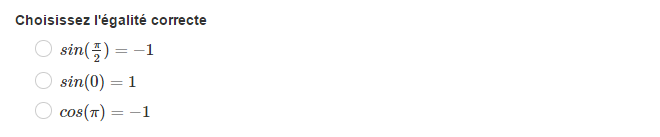
\includegraphics[width=0.800\linewidth]{radio.png}
\caption{QCM à boutons radio}\end{figure}


\subparagraph{Question à choix multiples avec plusieurs choix valides}
\label{doc-user:question-a-choix-multiples-avec-plusieurs-choix-valides}
Définie par la balise \code{\{++\}}, il s'agit d'une question semblable à la précédente mais l'élève a cette fois la possibilité de choisir plusieurs options. Les options qui doivent être sélectionnées sont définies avec la balise \code{\{=\}} et les autres avec la balise \code{\{*\}}. Le professeur doit cependant définir au moins une option correcte. Lors de la correction, l'élève peut obtenir des points pour un choix qu'il a coché et que le professeur a défini comme correct et inversement, c'est à dire qu'il peut aussi gagner des points sur un choix qui n'est pas sélectionné, à condition qu'il soit défini comme erroné.
\begin{figure}[htbp]
\centering
\capstart

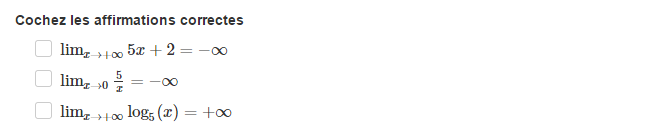
\includegraphics[width=0.800\linewidth]{checkbox.png}
\caption{QCM à cases à cocher}\end{figure}


\subsubsection{Affichage de l'aperçu et des erreurs}
\label{doc-user:affichage-de-l-apercu-et-des-erreurs}
Il est possible à tout moment d'afficher un rendu du quiz tel que le verront les étudiants en cliquant sur le bouton \emph{Aperçu} \textbf{(5)} en dessous de la zone de
texte. On peut ainsi voir si toutes les questions s'affichent comme prévu \textbf{(8)} et également détecter les éventuelles erreurs dans le code. Ces erreurs
apparaissent dans l'encadré rouge \textbf{(7)} en dessous du bouton \emph{Aperçu}. Pour chaque erreur, un message explicatif apparaît accompagné du numéro de ligne où s'est
produite l'erreur.

\begin{Verbatim}[commandchars=\\\{\}]
\PYGZob{}??\PYGZcb{} Résolution de l\PYGZsq{}équation suivante : 2x = 10
\PYGZob{}*=\PYGZcb{} x = 5
\PYGZob{}=r\PYGZcb{} Doit comporter le chiffre \PYGZdq{}5\PYGZdq{} // \PYGZca{}.*5.*\PYGZdl{}
\end{Verbatim}

Ici, on a tenté d'utiliser la balise \code{\{*=\}}, qui n'existe pas. C'est pourquoi on obtient le message suivant : \emph{Balise inconnue}.

Un quiz ne peut pas être envoyé et enregistré dans la base de données tant qu'il comporte encore des erreurs.


\subsubsection{Utilisation de Markdown pour la mise en forme}
\label{doc-user:utilisation-de-markdown-pour-la-mise-en-forme}
La mise en forme de certains éléments des quiz peut se faire avec du Markdown. Le Markdown est un langage de balisage à la syntaxe très
simple et intuitive. Il permet d'afficher d'afficher des titres, des liens, des images, des blocs du code ou encore de mettre du texte en gras ou en italique.
\href{https://guides.github.com/features/mastering-markdown/}{Ce tutoriel} \footnote{
\href{https://guides.github.com/features/mastering-markdown/}{https://guides.github.com/features/mastering-markdown/}. Consulté le 17 mai 2015.
} permet de prendre en main ce langage en quelques minutes.

Voici un exemple de question utilisant la mise en forme Markdown :

\begin{Verbatim}[commandchars=\\\{\}]
\PYGZob{}++\PYGZcb{}
\PYGZsh{}\PYGZsh{}\PYGZsh{} Titre de la question

Voici l\PYGZsq{}énoncé de la question. **Mot en gras**

{}`{}`{}`
def fonction():
    print(\PYGZdq{}Hello World\PYGZdq{})

    return True
{}`{}`{}`

[Tutoriel sur le markdown](https://guides.github.com/features/mastering\PYGZhy{}markdown/)
\PYGZob{}=\PYGZcb{} *Option en italique*
\PYGZob{}*\PYGZcb{} Code sur une ligne : {}`print(\PYGZdq{}Hello World\PYGZdq{}){}`
\end{Verbatim}

Une fois le rendu effectué, voici le résultat obtenu :
\begin{figure}[htbp]
\centering
\capstart

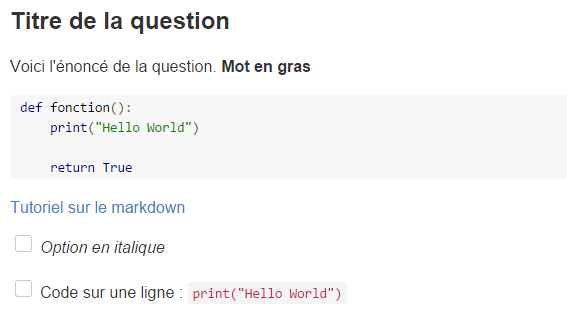
\includegraphics[width=0.800\linewidth]{markdown.png}
\caption{Mise en forme avec Markdown}\end{figure}

\begin{notice}{note}{Note:}
Il n'est pas nécessaire d'indiquer le langage utilisé pour afficher un bloc de code. Le langage est reconnu automatiquement
et la coloration syntaxique se fait en conséquence.
\end{notice}


\subsubsection{Affichage de mathématiques}
\label{doc-user:affichage-de-mathematiques}
Il est possible d'afficher des formules mathématiques à l'aide de la bibliothèque Javascript MathJax \footnote{
\href{http://www.mathjax.org/}{http://www.mathjax.org/}. Consulté le 29 mars 2015.
}. Cet outil permet d'écrire des expressions sous forme de LaTex et de les convertir en HTML pour qu'elles soient visibles dans le navigateur. Il existe deux méthodes d'affichage proposées par MathJax : la méthode \emph{in-line} et la méthode \emph{displayed}. La première méthode offre la possibilité d'inclure une formule dans un paragraphe de texte. Les formules en \emph{in-line} doivent être entourées des caractères suivants : \code{\textbackslash{}\textbackslash{}(...\textbackslash{}\textbackslash{})}. Avec la méthode \emph{displayed}, les expressions sont affichées en plus grand, centrées et détachées du reste du texte. Les formules utilisant cette méthode sont délimitées par les balises \code{\$\$...\$\$}.
\begin{figure}[htbp]
\centering
\capstart

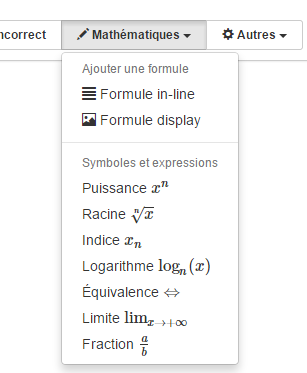
\includegraphics[width=0.400\linewidth]{math-menu.png}
\caption{Menu pour l'insertion de mathématiques}\end{figure}

La barre d'outils propose un menu dédié à l'affichage des mathématiques \textbf{(2)}. Deux boutons permettent d'insérer les délimiteurs des méthodes \emph{in-line} et \emph{displayed} et d'autres options pour afficher un échantillon de formules et de symboles sont disponibles. Cette liste est toutefois non-exhaustive.

Voici un exemple de question comportant l'affichage de limites :

\begin{Verbatim}[commandchars=\\\{\}]
\PYGZob{}++\PYGZcb{} Coche les affirmations correctes
\PYGZob{}*\PYGZcb{} \PYGZbs{}\PYGZbs{}(\PYGZbs{}lim\PYGZus{}\PYGZob{}x\PYGZbs{}to +\PYGZbs{}infty\PYGZcb{} 5x + 2 = \PYGZhy{}\PYGZbs{}infty\PYGZbs{}\PYGZbs{})
\PYGZob{}*\PYGZcb{} \PYGZbs{}\PYGZbs{}(\PYGZbs{}lim\PYGZus{}\PYGZob{}x\PYGZbs{}to 0\PYGZcb{} \PYGZbs{}frac\PYGZob{}5\PYGZcb{}\PYGZob{}x\PYGZcb{} = \PYGZhy{}\PYGZbs{}infty\PYGZbs{}\PYGZbs{})
\PYGZob{}=\PYGZcb{} \PYGZbs{}\PYGZbs{}(\PYGZbs{}lim\PYGZus{}\PYGZob{}x\PYGZbs{}to +\PYGZbs{}infty\PYGZcb{} \PYGZbs{}log\PYGZus{}\PYGZob{}5\PYGZcb{}(x) = +\PYGZbs{}infty\PYGZbs{}\PYGZbs{})
\end{Verbatim}

Résultat lors de l'aperçu :
\begin{figure}[htbp]
\centering
\capstart

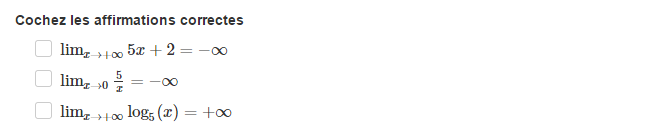
\includegraphics[width=0.700\linewidth]{checkbox.png}
\caption{Question avec des mathématiques}\end{figure}


\subsubsection{Enregistrement et importation de brouillons}
\label{doc-user:enregistrement-et-importation-de-brouillons}
Les brouillons permettent de stocker dans la base de données le code d'un quiz qui n'a pas encore été envoyé et de le récupérer plus tard pour terminer l'édition du quiz et le publier.

Le menu \emph{Brouillons} de la barre d'outils \textbf{(3)} est dédié à cette fonctionnalité.
\begin{figure}[htbp]
\centering
\capstart

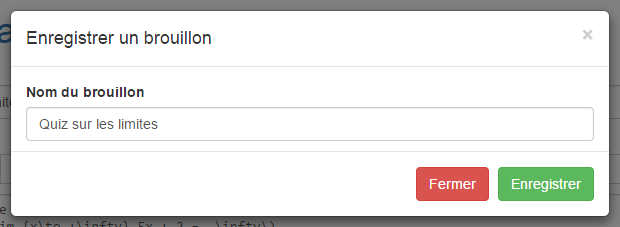
\includegraphics[width=0.700\linewidth]{draft-save.png}
\caption{Sauvegarde d'un brouillon}\end{figure}

Lorsqu'on clique sur le bouton \emph{Enregistrer un brouillon}, une boîte de dialogue apparaît. Il suffit de préciser un titre pour le brouillon et d'appuyer sur \emph{Enregistrer}. Un message confirmant que le brouillon a bien été enregistré apparaît.
\begin{figure}[htbp]
\centering
\capstart

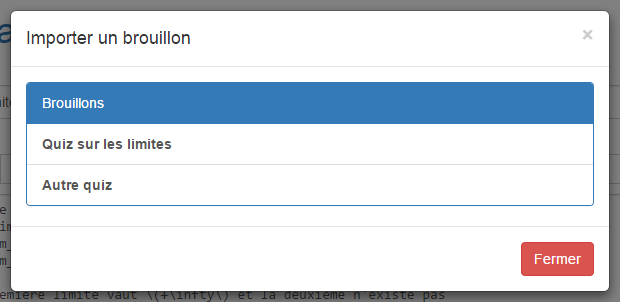
\includegraphics[width=0.700\linewidth]{draft-import.png}
\caption{Importation d'un brouillon}\end{figure}

Il est désormais possible d'importer ce brouillon grâce au bouton prévu à cet effet dans le menu. Une boîte de dialogue contenant la liste de tous les brouillons de l'utilisateur s'ouvre. Le brouillon recherché peut être importé par un simple clic. Le code du brouillon est alors inséré dans la zone de texte.


\subsubsection{Envoi définitif du quiz}
\label{doc-user:envoi-definitif-du-quiz}
Lorsque l'édition du quiz est terminée et que toutes les questions sont prêtes, le quiz peut être envoyé afin d'être sauvegardé dans la base de données et disponible à la résolution pour les élèves. Avant d'envoyer un quiz, il faut s'assurer d'avoir défini un titre \textbf{(1)} et d'avoir corrigé toutes les éventuelles erreurs présentes dans le code \textbf{(7)}. Lors du clic sur le bouton \emph{Enregistrer} \textbf{(6)}, un avertissement apparaîtra au cas où des erreurs persistent et l'envoi ne pourra pas se faire.


\subsection{Suivi des élèves}
\label{doc-user:suivi-des-eleves}

\subsubsection{Liste des quiz créés par un professeur}
\label{doc-user:liste-des-quiz-crees-par-un-professeur}\begin{figure}[htbp]
\centering
\capstart

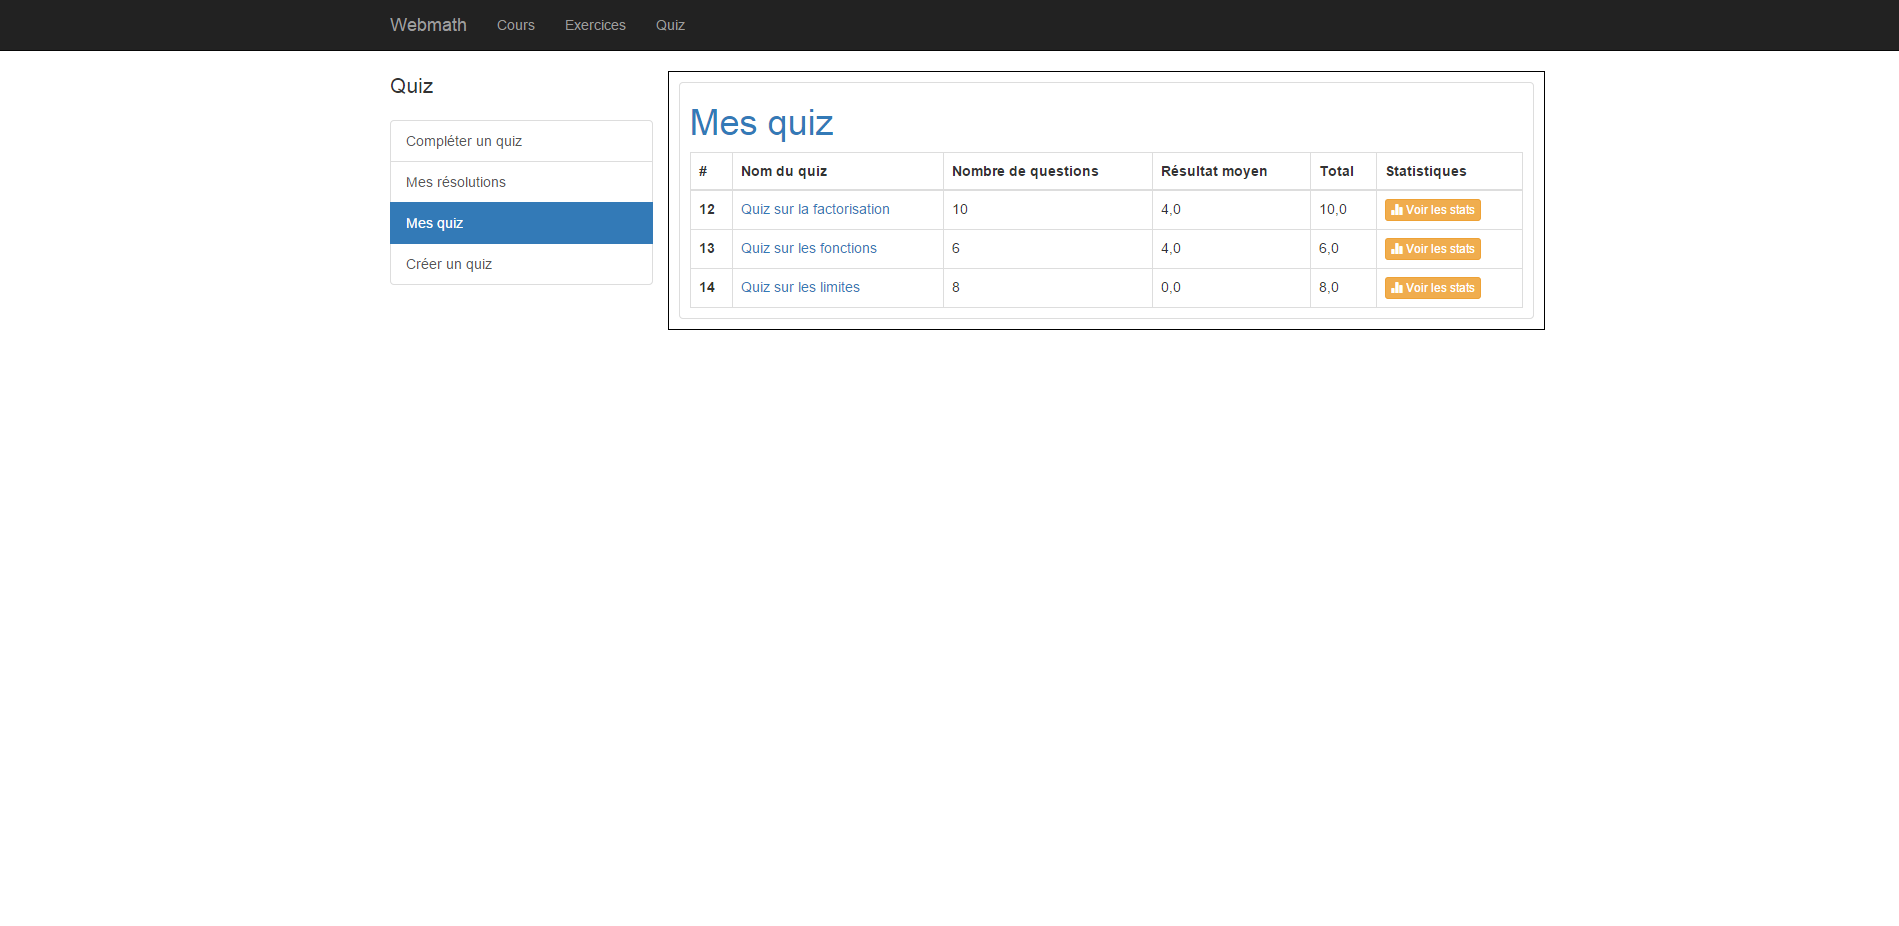
\includegraphics[width=0.700\linewidth]{my-quiz.png}
\caption{Liste des quiz créés par un professeur}\end{figure}

Dans l'onglet \emph{Mes quiz}, le professeur peut consulter la liste des quiz qu'il a créé avec des informations générales sur ceux-ci comme la moyenne de points obtenus pour chaque quiz. Grâce au bouton \emph{Voir les stats}, il peut accéder aux statistiques avancées d'un quiz en particulier.


\subsubsection{Affichage des statistiques avancées}
\label{doc-user:affichage-des-statistiques-avancees}\begin{figure}[htbp]
\centering
\capstart

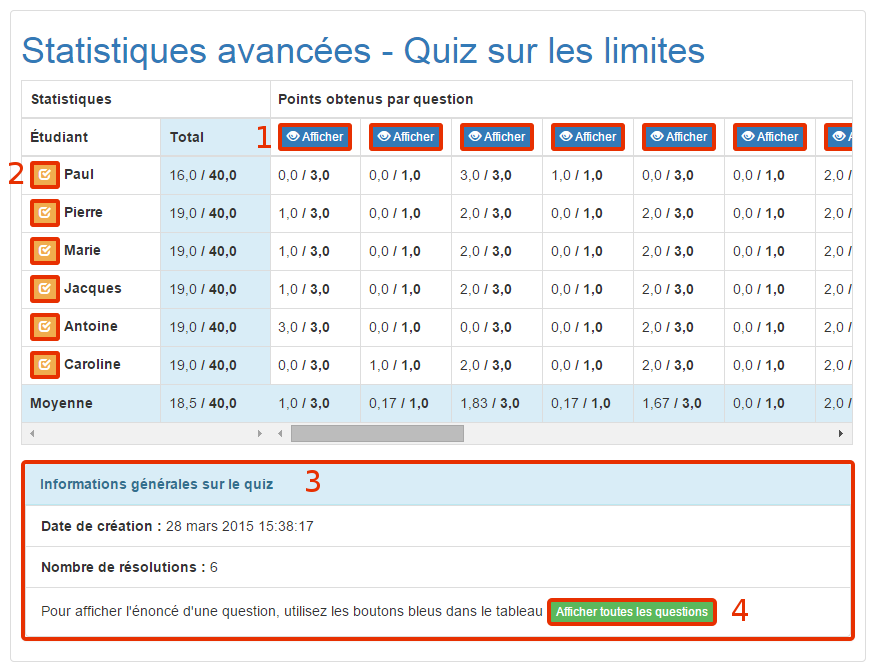
\includegraphics[width=0.700\linewidth]{stats.png}
\caption{Statistiques avancées}\end{figure}

Cette vue offre au professeur la possibilité de se faire une idée générale du niveau de compréhension des élèves d'un simple coup d'oeil. Pour chaque élève ayant répondu au quiz, il peut voir la note globale obtenue ainsi que les points attribués pour chaque question. Pour consulter les réponses soumises par un étudiant, le professeur peut cliquer sur le bouton orange situé au début de la colonne. Il sera ainsi redirigé vers la page de correction de la résolution.

Les boutons bleus \emph{Afficher} permettent de faire apparaître un aperçu rapide de chaque question. Toutes les questions du quiz peuvent aussi être consultées en même temps grâce au bouton \emph{Afficher toutes les questions}.

Lorsqu'on affiche une question à réponse courte, il est possible de voir les réponses soumises par les élèves qui n'ont pas répondu correctement. Le bouton rouge situé avant chaque réponse permet de valider une réponse et de l'ajouter aux solutions valides.
\begin{figure}[htbp]
\centering
\capstart

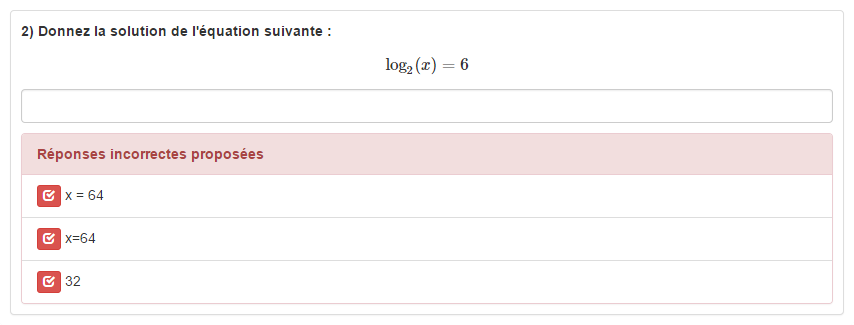
\includegraphics[width=0.700\linewidth]{add-solution.png}
\caption{Ajout d'une solution}\end{figure}

Ici, on voit que des étudiants ont trouvé la solution de l'équation mais l'ont simplement exprimé sous une autre forme que celle qui était attendue. Pour obtenir les points, ils auraient dû n'écrire que \code{64}. Après avoir cliqué sur le bouton, un message confirmant l'ajout de la solution apparaît, puis la couleur du bouton change. Les statistiques dans le tableau se mettent ensuite à jour. Désormais, tout élève écrivant la réponse sous cette forme-là obtiendra également les points pour la question.


\section{Étudiants}
\label{doc-user:etudiants}

\subsection{Trouver un quiz}
\label{doc-user:trouver-un-quiz}\begin{figure}[htbp]
\centering
\capstart

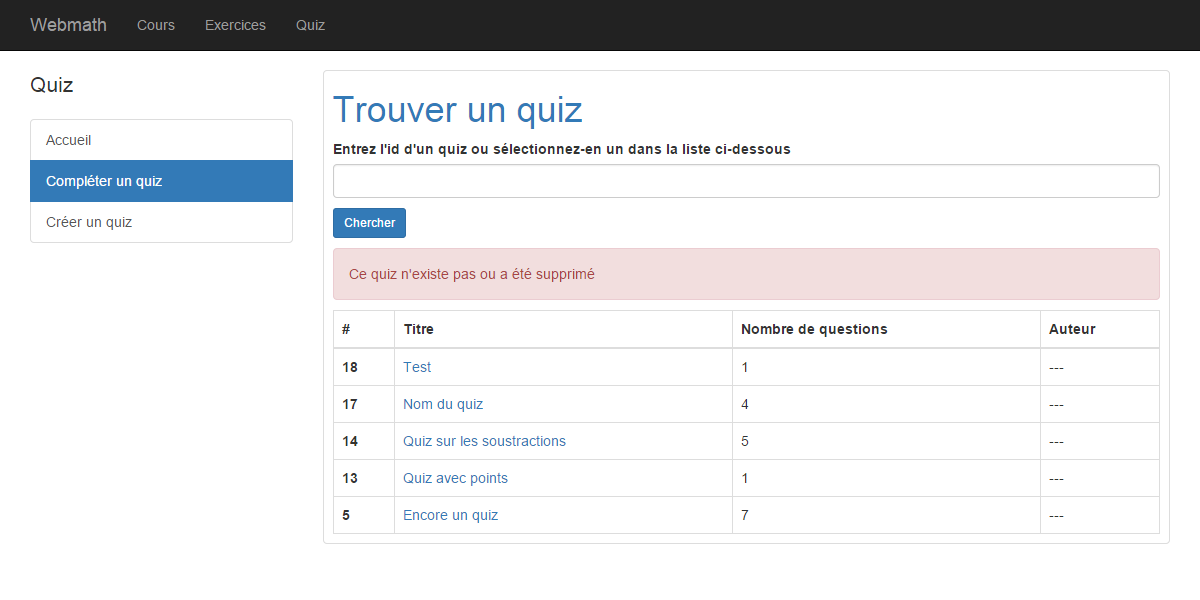
\includegraphics[width=0.700\linewidth]{find.png}
\caption{Page de recherche de quiz}\end{figure}

Pour trouver un quiz, un étudiant a plusieurs possibilités. Le professeur peut donner l'URL exacte du quiz à compléter, ce qui peut être pratique dans le cas d'un courriel ou toute autre communication informatisée. Un étudiant peut aussi accéder à un quiz en mémorisant son id et en l'entrant dans la champ prévu à cet effet dans l'onglet \emph{Compléter un quiz}.


\subsection{Compléter un quiz et correction automatique}
\label{doc-user:completer-un-quiz-et-correction-automatique}\begin{figure}[htbp]
\centering
\capstart

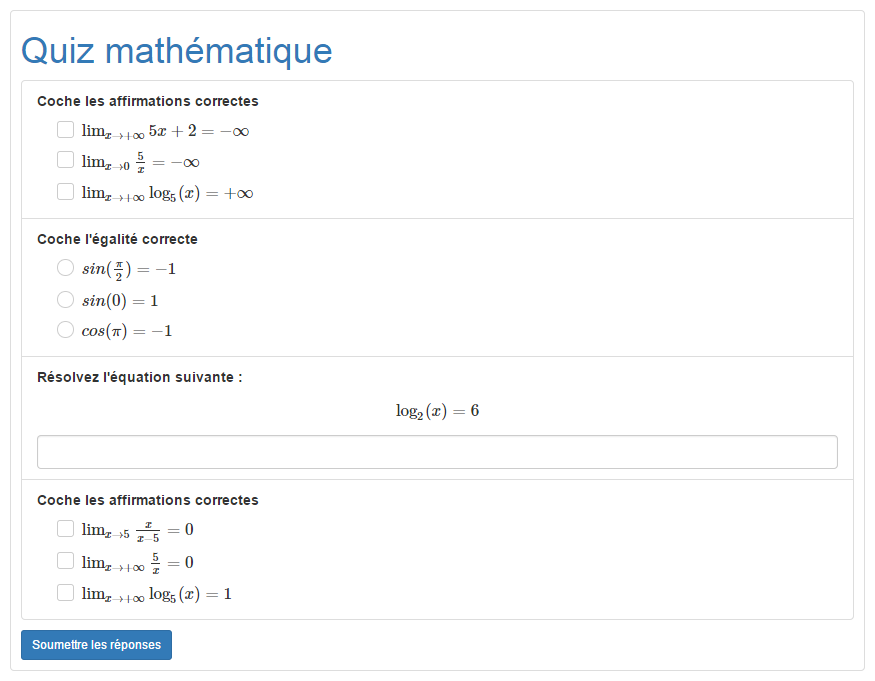
\includegraphics[width=0.700\linewidth]{complete.png}
\caption{Page pour compléter un quiz}\end{figure}

Une fois que l'étudiant a accédé au quiz, il peut le compléter très simplement en remplissant les champs de formulaires affichés. Lorsqu'il a fini, il peut soumettre ses réponses à l'aide du bouton prévu à cet effet. Les réponses soumises sont enregistrées dans la base de données et il est immédiatement redirigé vers une page de correction.

Les réponses incorrectes sont affichées en rouge avec la solution et une éventuelle explication donnée par le professeur pour chaque question. Les points reçus pour chaque question sont affichés avec le total de points sur le quiz. L'étudiant peut aussi comparer son score à la moyenne des autres étudiants qui ont complété le quiz.
\begin{figure}[htbp]
\centering
\capstart

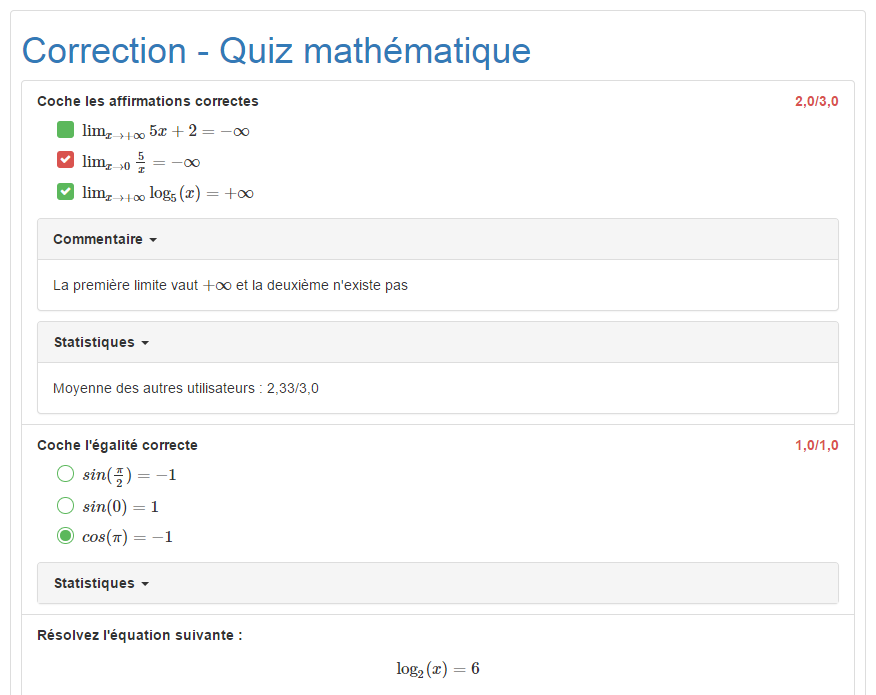
\includegraphics[width=0.700\linewidth]{correct.png}
\caption{Page de correction}\end{figure}

La page pour compléter un quiz ainsi que celle de la correction sont optimisées pour la navigation sur mobile et le design responsive s'adapte parfaitement à tous types de périphériques tels que les téléphones portables ou les tablettes, comme le montre la capture d'écran ci-dessous.
\begin{figure}[htbp]
\centering
\capstart

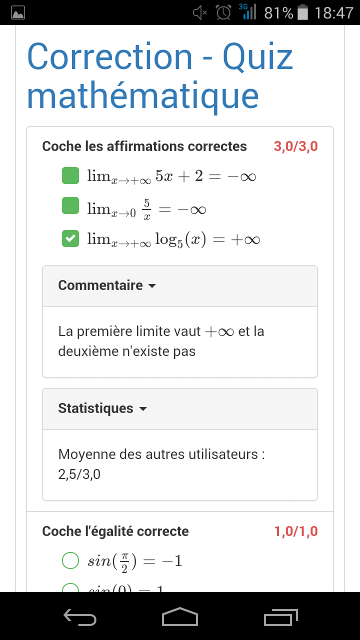
\includegraphics[width=0.400\linewidth]{mobile-1.png}
\caption{Page de correction sur mobile}\end{figure}


\subsection{Historique des résolutions}
\label{doc-user:historique-des-resolutions}\begin{figure}[htbp]
\centering
\capstart

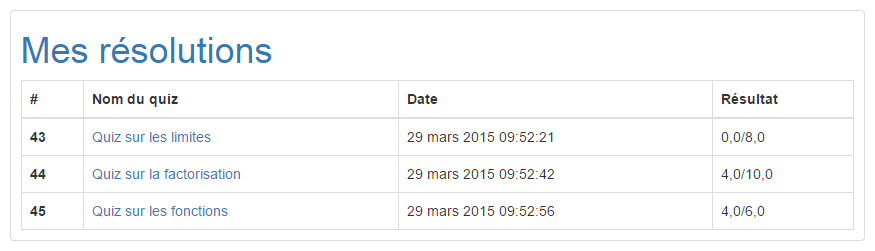
\includegraphics[width=0.700\linewidth]{completed.png}
\caption{Historique des résolutions de l'élève}\end{figure}

Les étudiants ont aussi la possibilité de garder une trace de tous les quiz qu'ils ont complétés. Dans l'onglet \emph{Mes résolutions} sont présentées toutes les résolutions apportées par l'élève à un quiz. Diverses informations complémentaires sont également disponibles, telles que la date et l'heure de la résolution ou le nombre de points obtenus. En cliquant sur un élément de la liste, l'étudiant est redirigé vers la page de correction de la résolution et peut ainsi voir les éventuelles erreurs qu'il a commises.


\chapter{Fonctionnement général de l'application}
\label{global::doc}\label{global:fonctionnement-general-de-l-application}

\section{URL}
\label{global:url}
Cette section définit les différents chemins d'accès aux pages de l'application. Certaines URL comportent des paramètres,
qui sont indiqués entre \textbf{\textless{}...\textgreater{}}. Les vues Django correspondant à chaque URL sont affichées entre parenthèses.
\begin{itemize}
\item {} 
\textbf{(find) :} Page d'accueil de l'application. Les étudiants peuvent voir les derniers quiz publiés ou en rechercher un.

\item {} 
\textbf{/create/ (create) :} Page de l'outil de création de quiz.

\item {} 
\textbf{/\textless{}id-quiz\textgreater{}/complete/ (complete) :} Page qui permet aux étudiants de répondre à un quiz et de soumettre leurs réponses.

\item {} 
\textbf{/\textless{}id-résolution\textgreater{}/correct/ (correct) :} Affichage de la correction d'une résolution. C'est là qu'est redirigé l'utilisateur après avoir complété un quiz

\item {} 
\textbf{/completed-quizzes/ (completed\_quizzes) :} Historique des résolutions effectuées par l'élève.

\item {} 
\textbf{/created-quizzes/ (created-quizzes) :} Liste des quiz créés par le professeur. C'est depuis cette page qu'il peut accéder aux statistiques avancées d'un quiz.

\item {} 
\textbf{/\textless{}id-quiz\textgreater{}/advanced-stats/ :} Affichage des statistiques avancées de toutes les résolutions d'un quiz.

\end{itemize}

D'autres URL sont utilisées uniquement par des requêtes Ajax, c'est à dire que l'utilisateur ne les voit jamais :
\begin{itemize}
\item {} 
\textbf{/findquiz/ (findquiz) :} Renvoie l'URL du quiz correspondant à la clé primaire du quiz fournie dans les paramètres de la requête HTTP si celui-ci existe.

\item {} 
\textbf{/savedraft/ (savedraft) :} Permet l'enregistrement dans la base de données d'un brouillon.

\item {} 
\textbf{/listdrafts/ (listdrafts) :} Récupère la liste des brouillons appartenant à l'utilisateur.

\item {} 
\textbf{/getdraft/ (getdraft) :} Récupère les données sur le brouillon dont la clé primaire est fournie dans les paramètres de la requête HTTP.

\item {} 
\textbf{/add-correct-answer/ (add\_correct\_answer) :} Pour une question à réponse courte, permet d'ajouter une réponse soumise aux solutions de la question

\end{itemize}

Voici comment sont définies ces URL dans Django :

\begin{Verbatim}[commandchars=\\\{\}]
\PYG{k+kn}{from} \PYG{n+nn}{django.conf.urls} \PYG{k+kn}{import} \PYG{n}{patterns}\PYG{p}{,} \PYG{n}{url}

\PYG{k+kn}{from} \PYG{n+nn}{quiz.views} \PYG{k+kn}{import} \PYG{o}{*}

\PYG{n}{urlpatterns} \PYG{o}{=} \PYG{n}{patterns}\PYG{p}{(}\PYG{l+s}{\PYGZsq{}}\PYG{l+s}{\PYGZsq{}}\PYG{p}{,}
    \PYG{c}{\PYGZsh{} URL des pages de l\PYGZsq{}application}
    \PYG{n}{url}\PYG{p}{(}\PYG{l+s}{r\PYGZsq{}}\PYG{l+s}{\PYGZca{}\PYGZdl{}}\PYG{l+s}{\PYGZsq{}}\PYG{p}{,} \PYG{n}{find}\PYG{p}{,} \PYG{n}{name}\PYG{o}{=}\PYG{l+s}{\PYGZdq{}}\PYG{l+s}{find}\PYG{l+s}{\PYGZdq{}}\PYG{p}{)}\PYG{p}{,}
    \PYG{n}{url}\PYG{p}{(}\PYG{l+s}{r\PYGZsq{}}\PYG{l+s}{\PYGZca{}create/\PYGZdl{}}\PYG{l+s}{\PYGZsq{}}\PYG{p}{,} \PYG{n}{create}\PYG{p}{,} \PYG{n}{name}\PYG{o}{=}\PYG{l+s}{\PYGZdq{}}\PYG{l+s}{create}\PYG{l+s}{\PYGZdq{}}\PYG{p}{)}\PYG{p}{,}
    \PYG{n}{url}\PYG{p}{(}\PYG{l+s}{r\PYGZsq{}}\PYG{l+s}{\PYGZca{}(}\PYG{l+s}{\PYGZbs{}}\PYG{l+s}{d+)/complete/}\PYG{l+s}{\PYGZsq{}}\PYG{p}{,} \PYG{n}{complete}\PYG{p}{,} \PYG{n}{name}\PYG{o}{=}\PYG{l+s}{\PYGZdq{}}\PYG{l+s}{complete}\PYG{l+s}{\PYGZdq{}}\PYG{p}{)}\PYG{p}{,}
    \PYG{n}{url}\PYG{p}{(}\PYG{l+s}{r\PYGZsq{}}\PYG{l+s}{\PYGZca{}(}\PYG{l+s}{\PYGZbs{}}\PYG{l+s}{d+)/correct/}\PYG{l+s}{\PYGZsq{}}\PYG{p}{,} \PYG{n}{correct}\PYG{p}{,} \PYG{n}{name}\PYG{o}{=}\PYG{l+s}{\PYGZdq{}}\PYG{l+s}{correct}\PYG{l+s}{\PYGZdq{}}\PYG{p}{)}\PYG{p}{,}
    \PYG{n}{url}\PYG{p}{(}\PYG{l+s}{r\PYGZsq{}}\PYG{l+s}{\PYGZca{}completed\PYGZhy{}quizzes/}\PYG{l+s}{\PYGZsq{}}\PYG{p}{,} \PYG{n}{completed\PYGZus{}quizzes}\PYG{p}{,} \PYG{n}{name}\PYG{o}{=}\PYG{l+s}{\PYGZdq{}}\PYG{l+s}{completed\PYGZhy{}quizzes}\PYG{l+s}{\PYGZdq{}}\PYG{p}{)}\PYG{p}{,}
    \PYG{n}{url}\PYG{p}{(}\PYG{l+s}{r\PYGZsq{}}\PYG{l+s}{\PYGZca{}created\PYGZhy{}quizzes/}\PYG{l+s}{\PYGZsq{}}\PYG{p}{,} \PYG{n}{created\PYGZus{}quizzes}\PYG{p}{,} \PYG{n}{name}\PYG{o}{=}\PYG{l+s}{\PYGZdq{}}\PYG{l+s}{created\PYGZhy{}quizzes}\PYG{l+s}{\PYGZdq{}}\PYG{p}{)}\PYG{p}{,}
    \PYG{n}{url}\PYG{p}{(}\PYG{l+s}{\PYGZsq{}}\PYG{l+s}{\PYGZca{}(}\PYG{l+s}{\PYGZbs{}}\PYG{l+s}{d+)/advanced\PYGZhy{}stats/}\PYG{l+s}{\PYGZsq{}}\PYG{p}{,} \PYG{n}{advanced\PYGZus{}stats}\PYG{p}{,} \PYG{n}{name}\PYG{o}{=}\PYG{l+s}{\PYGZdq{}}\PYG{l+s}{advanced\PYGZhy{}stats}\PYG{l+s}{\PYGZdq{}}\PYG{p}{)}\PYG{p}{,}
    \PYG{c}{\PYGZsh{} URL destinées à l\PYGZsq{}Ajax}
    \PYG{n}{url}\PYG{p}{(}\PYG{l+s}{r\PYGZsq{}}\PYG{l+s}{\PYGZca{}findquiz/}\PYG{l+s}{\PYGZsq{}}\PYG{p}{,} \PYG{n}{findquiz}\PYG{p}{,} \PYG{n}{name}\PYG{o}{=}\PYG{l+s}{\PYGZdq{}}\PYG{l+s}{findquiz}\PYG{l+s}{\PYGZdq{}}\PYG{p}{)}\PYG{p}{,}
    \PYG{n}{url}\PYG{p}{(}\PYG{l+s}{r\PYGZsq{}}\PYG{l+s}{\PYGZca{}savedraft/}\PYG{l+s}{\PYGZsq{}}\PYG{p}{,} \PYG{n}{savedraft}\PYG{p}{,} \PYG{n}{name}\PYG{o}{=}\PYG{l+s}{\PYGZdq{}}\PYG{l+s}{savedraft}\PYG{l+s}{\PYGZdq{}}\PYG{p}{)}\PYG{p}{,}
    \PYG{n}{url}\PYG{p}{(}\PYG{l+s}{r\PYGZsq{}}\PYG{l+s}{\PYGZca{}listdrafts/}\PYG{l+s}{\PYGZsq{}}\PYG{p}{,} \PYG{n}{listdrafts}\PYG{p}{,} \PYG{n}{name}\PYG{o}{=}\PYG{l+s}{\PYGZdq{}}\PYG{l+s}{listdrafts}\PYG{l+s}{\PYGZdq{}}\PYG{p}{)}\PYG{p}{,}
    \PYG{n}{url}\PYG{p}{(}\PYG{l+s}{r\PYGZsq{}}\PYG{l+s}{\PYGZca{}getdraft/}\PYG{l+s}{\PYGZsq{}}\PYG{p}{,} \PYG{n}{getdraft}\PYG{p}{,} \PYG{n}{name}\PYG{o}{=}\PYG{l+s}{\PYGZdq{}}\PYG{l+s}{getdraft}\PYG{l+s}{\PYGZdq{}}\PYG{p}{)}\PYG{p}{,}
    \PYG{n}{url}\PYG{p}{(}\PYG{l+s}{r\PYGZsq{}}\PYG{l+s}{\PYGZca{}add\PYGZhy{}correct\PYGZhy{}answer/}\PYG{l+s}{\PYGZsq{}}\PYG{p}{,} \PYG{n}{add\PYGZus{}correct\PYGZus{}answer}\PYG{p}{,} \PYG{n}{name}\PYG{o}{=}\PYG{l+s}{\PYGZdq{}}\PYG{l+s}{add\PYGZhy{}correct\PYGZhy{}answer}\PYG{l+s}{\PYGZdq{}}\PYG{p}{)}\PYG{p}{,}
\PYG{p}{)}
\end{Verbatim}

Chaque URL est définie à l'aide de la fonction \code{url()}. Cette fonction prend trois arguments : une expression régulière qui
caractérise l'URL, la référence de la fonction correspondante dans les vues ainsi que le nom de l'URL, qui pourra être utilisé
avec la fonction \code{reverse()} pour construire un lien vers une page de l'application.


\section{Organisation des fichiers de l'application}
\label{global:organisation-des-fichiers-de-l-application}
Ce chapitre décrit tous les dossiers et fichiers importants de l'application ainsi que leur rôle dans le fonctionnement du site.
\begin{itemize}
\item {} 
\textbf{admin.py :} Fichier qui permet de personnaliser l'interface d'administration de l'application.

\item {} 
\textbf{forms.py :} Définit les formulaires Django personnalisés utilisés dans l'application.application.

\item {} 
\textbf{models.py :} Décrit les modèles de l'application, c'est à dire les tables de la base de données.

\item {} 
\textbf{urls.py :} Définit les chemins d'accès pour les différentes pages de l'application.

\item {} 
\textbf{views.py :} Les vues Django de l'application, c'est à dire un ensemble de fonctions qui définissent les actions à réaliser lorsqu'un utilisateur tente d'accéder à une page.

\item {} 
\textbf{migrations/ :} Ce dossier contient des fichiers Python générés par Django qui gèrent les modifications apportées aux tables de la base de données.

\item {} 
\textbf{rs-source/ :} Dossier contenant tout le code écrit en RapydScript utilisé dans l'application.
\begin{itemize}
\item {} 
\textbf{find\_url.pyj :} Gère la requête Ajax pour rechercher un quiz à compléter.

\item {} 
\textbf{interpreter.pyj :} Permet d'interpréter le code de l'outil de création de quiz pour structurer les données du quiz en JSON.

\item {} 
\textbf{Makefile :} Définit des raccourcis pour la compilation des fichiers RapydScript

\item {} 
\textbf{toolbar.pyj :} Implémente les différentes fonctionalités de la barre d'outils de la page de création de quiz.

\end{itemize}

\item {} 
\textbf{static/quiz/ :} Contient tous les fichiers statiques de l'application
\begin{itemize}
\item {} 
\textbf{css/ :} Fichiers CSS
\begin{itemize}
\item {} 
\textbf{awesome-checkbox/ :} Répertoire contenant les fichiers du plugin \href{https://github.com/flatlogic/awesome-bootstrap-checkbox}{Awesome Bootstrap Checkbox} \footnote{
\href{https://github.com/flatlogic/awesome-bootstrap-checkbox}{https://github.com/flatlogic/awesome-bootstrap-checkbox}. Consulté le 29 mars 2015.
} pour mettre en forme les boutons radio et les cases à cocher.

\item {} 
\textbf{create.css :} Feuille de style spécifique à la page de création de quiz

\item {} 
\textbf{shop-item.css :} Feuille de style relative au template \href{http://startbootstrap.com/template-overviews/shop-item/}{Shop Item} \footnote{
\href{http://startbootstrap.com/template-overviews/shop-item/}{http://startbootstrap.com/template-overviews/shop-item/}. Consulté le 29 mars 2015.
} utilisé dans toute l'application.

\item {} 
\textbf{stas.css :} Feuille de style spécifique à la page de statistiques avancées.

\item {} 
\textbf{style.css :} Feuille de style qui s'applique à l'ensemble de l'application.

\item {} 
\textbf{github-markdown.css :} Feuille de style pour mettre en forme le HTML généré à partir du Markdown de manière similaire à Github \footnote{
\href{https://github.com/sindresorhus/github-markdown-css}{https://github.com/sindresorhus/github-markdown-css}. Consulté le 17 mai 2015.
}

\item {} 
\textbf{showdown.js :} Fichier de la bibliothèque Javascript Showdown \footnote{
\href{https://github.com/showdownjs/showdown}{https://github.com/showdownjs/showdown}. Consulté le 17 mai 2015.
}

\end{itemize}

\item {} 
\textbf{js/ :} Fichiers Javascript
\begin{itemize}
\item {} 
\textbf{rs-compiled/ :} Dossier contenant les fichiers RapydScript compilés.

\item {} 
\textbf{jquery.caret.js :} Plugin \href{https://github.com/acdvorak/jquery.caret}{jQuery Caret} \footnote{
\href{https://github.com/acdvorak/jquery.caret}{https://github.com/acdvorak/jquery.caret}. Consulté le 29 mars 2015.
} pour récupérer la position du curseur dans une zone de texte.

\item {} 
\textbf{stats.js :} Définit une requête Ajax pour ajouter des solutions à une question dans la page de statistiques.

\item {} 
\textbf{textarea\_lines.js :} Script pour afficher les numéros de ligne dynamiquement dans une zone de texte.

\item {} 
\textbf{utils.js :} Fichier comportant différentes fonctions utiles à différents endroits de l'application.

\end{itemize}

\end{itemize}

\item {} 
\textbf{templates/quiz/ :} Dossier contenant les gabarits de l'application. Hormis \textbf{base.html}, chaque fichier de ce répertoire correspond à la vue Django du même nom.
\begin{itemize}
\item {} 
\textbf{base.html :} Gabarit global de l'application dont héritent tous les autres gabarits.

\end{itemize}

\item {} 
\textbf{utils/ :} Contient des modules Python utilisés dans les vues.
\begin{itemize}
\item {} 
\textbf{correct.py :} Définit des objets utiles pour l'affichage de la correction.

\item {} 
\textbf{save.py :} Gère l'enregistrement des quiz dans la base de données.

\item {} 
\textbf{submit.py :} Gère la sauvegarde des réponses soumises à un quiz par un étudiant.

\end{itemize}

\end{itemize}


\section{Bibliothèques et frameworks utilisés dans l'application}
\label{global:bibliotheques-et-frameworks-utilises-dans-l-application}
Voici la liste des outils provenant de sources extérieures utilisés dans le projet
\begin{itemize}
\item {} 
Django \footnote{
\href{https://djangoproject.com}{https://djangoproject.com}. Consulté le 29 mars 2015.
} : framework Python pour créer des sites web dynamiques.

\item {} 
RapydScript \footnote{
\href{http://rapydscript.pyjeon.com/}{http://rapydscript.pyjeon.com/}. Consulté le 29 mars 2015.
} : outil pour compiler du Python en Javascript.

\item {} 
Bootstrap \footnote{
\href{http://getbootstrap.com/}{http://getbootstrap.com/}. Consulté le 29 mars 2015.
} : framwork CSS pour avoir un affichage correct très rapidement.

\item {} 
jQuery \footnote{
\href{https://jquery.com/}{https://jquery.com/}. Consulté le 29 mars 2015.
} : bibliothèque Javascript pour les manipulations dans le DOM, requêtes Ajax, etc.

\item {} 
MathJax \footnote{
\href{http://www.mathjax.org/}{http://www.mathjax.org/}. Consulté le 29 mars 2015.
} : bibliothèque Javascript permettant l'affichage de mathématiques.

\item {} 
Awesome Bootstrap Checkbox \footnotemark[12] : feuille de style pour les cases à cocher et les boutons radio.

\item {} 
jQuery Caret \footnotemark[14] : plugin jQuery pour récupérer la position du curseur dans une zone de texte.

\item {} 
Shop Item \footnotemark[13] : gabarit bootstrap utilisé dans toute l'application.

\item {} 
Showdown \footnotemark[20] : bibliothèque Javascript pour générer du HTML à partir de Markdown.

\item {} 
Github Markdown CSS \footnotemark[21] : Feuille de style pour mettre en forme le HTML généré à partir du Markdown de manière similaire à Github.

\item {} 
Google Code Prettify \footnote{
\href{https://github.com/google/code-prettify}{https://github.com/google/code-prettify}. Consulté le 17 mai 2015.
} : script pour la coloration syntaxique du code affiché avec le Markdown.

\end{itemize}


\chapter{Modèle relationnel}
\label{database::doc}\label{database:modele-relationnel}

\section{Introduction}
\label{database:introduction}
Une des premières étapes importantes dans le développement d'un site web est l'élaboration d'un modèle relationnel structuré permettant de stocker toutes les données générées par l'application et de les relier entre elles. Un modèle relationnel décrit les différentes tables de la base de données et les liens entre ces tables. Une table peut être comparée à un tableau contenant des informations. Chaque table comporte une ou plusieurs colonnes, chaque colonne stockant un type de données précisément défini, par exemple un nombre entier ou une chaîne de caractères. Si on imagine une table contenant les données sur les utilisateurs d'un site, une colonne pourrait alors contenir le pseudonyme d'un utilisateur et une autre son âge. On peut ensuite ajouter des entrées dans une table, c'est à dire un ensemble de données dont chaque élément correspond à une colonne de la table. Dans l'exemple précédent, on ajouterait ainsi une ligne pour chaque utilisateur s'inscrivant sur le site. Chaque ligne est identifiée grâce à une clé primaire unique, habituellement sous la forme d'un entier, qui permet de créer des liens entre différentes lignes de différentes tables. Ces liens entre différentes tables sont appelées relations.

Voici, présenté sous forme simplifiée à l'aide d'un tableau, comment on pourrait stocker les données concernant des quiz et leurs créateurs :

\textbf{Table contenant les utilisateurs :}

\begin{tabulary}{\linewidth}{|L|L|L|}
\hline
\textsf{\relax 
Clé primaire
} & \textsf{\relax 
Prénom
} & \textsf{\relax 
Âge
}\\
\hline
1
 & 
Paul
 & 
26
\\
\hline
2
 & 
Juliette
 & 
22
\\
\hline
3
 & 
Marc
 & 
48
\\
\hline\end{tabulary}


\textbf{Table contenant les quiz :}

\begin{tabulary}{\linewidth}{|L|L|L|}
\hline
\textsf{\relax 
Clé primaire
} & \textsf{\relax 
Titre du quiz
} & \textsf{\relax 
Auteur
}\\
\hline
1
 & 
Fonctions exponentielles
 & 
3
\\
\hline
2
 & 
Logarithmes
 & 
3
\\
\hline
3
 & 
Comportement à l'infini
 & 
2
\\
\hline\end{tabulary}


Ici, le premier quiz a comme titre \emph{Fonctions exponentielles}, comporte 5 questions et a été créé par Marc (Utilisateur 3).

Une fois que le modèle relationnel a été élaboré, on peut créer une base de données sous forme de fichier. Le langage SQL permet de créer les tables d'une base de données, d'y enregistrer des informations et de faire des requêtes, c'est à dire récupérer des données enregistrées. Un logiciel ou une application web peut ainsi communiquer avec une base de données et stocker les informations nécessaires de manière permanente.

Django offre la possibilité de créer une base de données et d'interagir avec celle-ci par le biais d'une ORM (Object Relational Mapper), on peut donc éviter l'utilisation du langage SQL et communiquer avec la base de données avec des objets et des méthodes Python. Cet aspect de Django sera abordé un peu plus loin.


\section{Utilisation dans l'application de création de quiz}
\label{database:utilisation-dans-l-application-de-creation-de-quiz}

\subsection{Implémentation dans Django}
\label{database:implementation-dans-django}
Comme indiqué précédemment, Django fournit une interface de haut niveau pour créer et interagir avec une base de données. On peut écrire nos tables avec une architecture orientée objet, que Django ``traduira'' ensuite en SQL. Ainsi, pour créer une table dans notre base de données, il suffit de définir une classe héritant de \code{models.Model} et d'initialiser des variables de classes pour ajouter des colonnes à la table. Ainsi, par exemple, pour implémenter une table contenant les données générales d'un quiz, il suffit d'écrire le code suivant :

\begin{Verbatim}[commandchars=\\\{\}]
\PYG{k}{class} \PYG{n+nc}{Quiz}\PYG{p}{(}\PYG{n}{models}\PYG{o}{.}\PYG{n}{Model}\PYG{p}{)}\PYG{p}{:} \PYG{c}{\PYGZsh{}Infos générales sur le quiz}
    \PYG{n}{title} \PYG{o}{=} \PYG{n}{models}\PYG{o}{.}\PYG{n}{CharField}\PYG{p}{(}\PYG{n}{max\PYGZus{}length}\PYG{o}{=}\PYG{l+m+mi}{100}\PYG{p}{)} \PYG{c}{\PYGZsh{}Colonne contenant une chaîne de caractères}
    \PYG{n}{creation\PYGZus{}date} \PYG{o}{=} \PYG{n}{models}\PYG{o}{.}\PYG{n}{DateTimeField}\PYG{p}{(}\PYG{p}{)} \PYG{c}{\PYGZsh{}Colonne contenant une date/heure}
    \PYG{n}{code} \PYG{o}{=} \PYG{n}{models}\PYG{o}{.}\PYG{n}{CharField}\PYG{p}{(}\PYG{n}{max\PYGZus{}length}\PYG{o}{=}\PYG{l+m+mi}{1000}\PYG{p}{)} \PYG{c}{\PYGZsh{}Colonne contenant une chaîne de caractères}
\end{Verbatim}

Les objets comme \code{CharField()} ou \code{DateTimeField()} permettent de définir des champs d'un type de données précis. Une liste complète des types de champs est disponible sur \href{https://docs.djangoproject.com/en/1.7/ref/models/fields/\#field-types}{la documentation officielle de Django} \footnote{
\href{https://docs.djangoproject.com/en/1.7/ref/models/fields/\#field-types}{https://docs.djangoproject.com/en/1.7/ref/models/fields/\#field-types}. Consulté le 29 mars 2015.
}


\subsection{Schéma global}
\label{database:schema-global}
L'élaboration d'un schéma relationnel n'est pas chose facile car il est nécessaire que celui-ci réponde à certains critères. Il doit être relativement simple afin de garder une certaine flexibilité pour pouvoir être modifié plus tard, car il est souvent difficile de prédire à l'avance les difficultés liées au stockage des données qui pourraient être rencontrées au cours du développement. Il doit également être possible d'ajouter des fonctionnalités sans devoir revoir toute l'organisation du schéma ou créer un trop grand nombre de nouvelles tables. Malgré cela, le modèle doit aussi correspondre aux exigences des fonctionnalités de l'application et doit inclure toutes les relations nécessaires. Il s'agit donc d'une étape cruciale qui peut s'avérer décisive pour la suite du développement.

Voici le diagramme des tables utilisés pour stocker les données des quiz :
\begin{figure}[htbp]
\centering

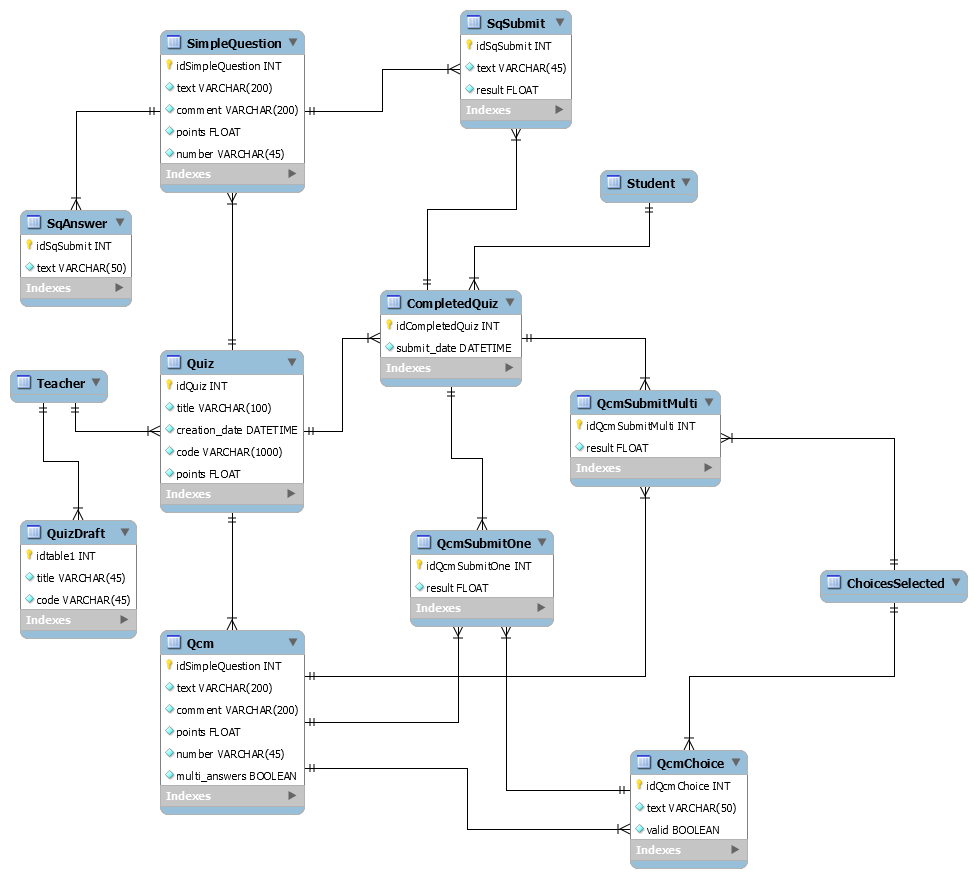
\includegraphics{quiz-models.png}
\end{figure}


\subsection{Explications des tables}
\label{database:explications-des-tables}
Dans ce chapitre sont présentés tous les modèles définis dans le fichier \emph{models.py}.
L'utilisation d'une architecture orientée objet pour la création de tables dans la base
de données permet l'utilisation de méthodes, qui se révèlent très pratiques lorsqu'on
veut récupérer des informations équivalentes depuis des éléments provenant de tables
différentes. Par exemple, si on veut afficher le résultat moyen obtenu pour chacune
des questions d'un quiz, il est très intéressant de pouvoir appliquer la même méthode
à toutes les questions pour récupérer leur moyenne sans se soucier de la classe à laquelle
ces questions appartiennent.
\index{Quiz (classe dans quiz.models)}

\begin{fulllineitems}
\phantomsection\label{database:quiz.models.Quiz}\pysiglinewithargsret{\strong{class }\code{quiz.models.}\bfcode{Quiz}}{\emph{*args}, \emph{**kwargs}}{}
La table \code{Quiz} est la table centrale de l'application et toutes les autres 
tables s'organisent autour d'elle. Elle comporte trois colonnes importantes :
une contenant le titre, une autre contenant la date et l'heure de création 
ainsi qu'une colonne 
dans laquelle est stockée le nombre maximal de points pouvant être obtenus pour
le quiz en question. Cette table comporte également une relation vers une table
Teacher  qui permet d'intégrer le système d'authentification des utilisateurs.

Avec django, il est possible d'initialiser automatiquement un champ \code{DateTimeField} à la date/heure du moment où le modèle est instancié avec le paramètre \code{auto\_now\_add}

\begin{Verbatim}[commandchars=\\\{\}]
\PYG{n}{creation\PYGZus{}date} \PYG{o}{=} \PYG{n}{models}\PYG{o}{.}\PYG{n}{DateTimeField}\PYG{p}{(}\PYG{n}{auto\PYGZus{}now\PYGZus{}add}\PYG{o}{=}\PYG{n+nb+bp}{True}\PYG{p}{)}
\end{Verbatim}
\index{average\_result() (méthode quiz.models.Quiz)}

\begin{fulllineitems}
\phantomsection\label{database:quiz.models.Quiz.average_result}\pysiglinewithargsret{\bfcode{average\_result}}{}{}
Récupère dans la base de données toutes les résolutions se rattachant
au quiz en question puis calcule la moyenne des résultats obtenus sur la base
du résultat de chaque élève et le nombre de résolutions envoyées.

\end{fulllineitems}

\index{get\_questions() (méthode quiz.models.Quiz)}

\begin{fulllineitems}
\phantomsection\label{database:quiz.models.Quiz.get_questions}\pysiglinewithargsret{\bfcode{get\_questions}}{}{}
Récupère la liste de toutes les questions du quiz et les trie dans l'ordre
d'apparition dans le quiz.

\end{fulllineitems}

\index{length() (méthode quiz.models.Quiz)}

\begin{fulllineitems}
\phantomsection\label{database:quiz.models.Quiz.length}\pysiglinewithargsret{\bfcode{length}}{}{}
Retourne le nombre de questions qui composent le quiz.

\end{fulllineitems}


\end{fulllineitems}

\index{CompletedQuiz (classe dans quiz.models)}

\begin{fulllineitems}
\phantomsection\label{database:quiz.models.CompletedQuiz}\pysiglinewithargsret{\strong{class }\code{quiz.models.}\bfcode{CompletedQuiz}}{\emph{*args}, \emph{**kwargs}}{}
Comme on peut le voir sur le diagramme, à l'instar de \code{Quiz}, cette table
occupe aussi un rôle central dans le modèle relationnel. Elle permet de faire
le lien entre un quiz créé par un professeur et les réponses soumises à ce quiz
par les étudiants. Elle possède donc une relation vers une table \code{Student},
qui définit l'étudiant ayant répondu au quiz. De l'autre côté, cette table pointe
vers \code{Quiz} et définit logiquement le quiz auquel l'étudiant a répondu. Un seul
champ est présent : la date et l'heure de la soumission des réponses.
\index{get\_questions\_submits() (méthode quiz.models.CompletedQuiz)}

\begin{fulllineitems}
\phantomsection\label{database:quiz.models.CompletedQuiz.get_questions_submits}\pysiglinewithargsret{\bfcode{get\_questions\_submits}}{}{}
Renvoie la liste des entrées des tables \code{SqSubmit}, \code{QcmSubmitOne} et
\code{QcmSubmitMulti} correspondant à la résolution \code{self}.
Chaque élément de cette liste représente concrètement la réponse soumise à
une question du quiz.

Cette liste est triée selon l'ordre d'apparition des questions correspondant
réponses proposées.

\end{fulllineitems}

\index{update\_total\_result() (méthode quiz.models.CompletedQuiz)}

\begin{fulllineitems}
\phantomsection\label{database:quiz.models.CompletedQuiz.update_total_result}\pysiglinewithargsret{\bfcode{update\_total\_result}}{}{}
Met à jour le nombre de points obtenus pour la résolution du quiz en entier
en fonction des points obtenus pour chaque réponse soumise aux questions
du quiz.

Pour comptabiliser le nombre total de points obtenus, cette méthode parcourt
la liste des réponses apportées avec la méthode \code{.get\_questions\_submits()}
appliquée à la résolution en question.

Cette méthode peut être utilisée lorsqu'une résolution vient d'être soumise
par un élève pour comptabiliser une première fois les points obtenus ou 
lorsqu'une entrée dans \code{SqAnswer} a été ajoutée pour mettre à jour les
statistiques en fonction des changements.

\end{fulllineitems}


\end{fulllineitems}

\index{QuizDraft (classe dans quiz.models)}

\begin{fulllineitems}
\phantomsection\label{database:quiz.models.QuizDraft}\pysiglinewithargsret{\strong{class }\code{quiz.models.}\bfcode{QuizDraft}}{\emph{*args}, \emph{**kwargs}}{}
Cette table est un peu isolée dans le schéma relationnel et n'a qu'une fonction :
enregistrer le code qu'un quiz qu'un professeur n'a pas terminé et lui offrir
la possibilité de le récupérer plus tard pour continuer son travail.
Outre la relation vers la table \code{Teacher} et la colonne stockant le code du
quiz, une colonne permet de stocker un titre pour pouvoir identifier rapidement
un brouillon.

\end{fulllineitems}

\index{SimpleQuestion (classe dans quiz.models)}

\begin{fulllineitems}
\phantomsection\label{database:quiz.models.SimpleQuestion}\pysiglinewithargsret{\strong{class }\code{quiz.models.}\bfcode{SimpleQuestion}}{\emph{*args}, \emph{**kwargs}}{}
Cette table contient les informations générales sur les questions simples du quiz.
Ces questions sont présentées sous la forme d'un simple champ de texte lorsqu'un
élève complète le quiz. Une première colonne \code{title} stocke l'énoncé de la
question, \code{comment} permet d'inclure un commentaire affiché lors de la
correction automatique du quiz (par exemple la démonstration d'une égalité),
\code{points} définit le nombre de points attribués sur cette question et \code{number}
enregistre la position à laquelle doit apparaître la question dans le quiz. Une relation
désigne le quiz qui intègre la question.
\index{average\_result() (méthode quiz.models.SimpleQuestion)}

\begin{fulllineitems}
\phantomsection\label{database:quiz.models.SimpleQuestion.average_result}\pysiglinewithargsret{\bfcode{average\_result}}{}{}
Renvoie le nombre moyen de points obtenus pour la question en se basant sur
le nombre total de réponses soumises et sur la somme de tous les points obtenus.
La moyenne est ensuite arrondie à deux chiffres après la virgule pour éviter
tout problème d'affichage.

Au cas où aucune réponse n'a encore été soumise, cette méthode retourne
simplement la chaîne \code{-{-}} qui peut directement être utilisée dans le template.

\end{fulllineitems}

\index{create\_form() (méthode quiz.models.SimpleQuestion)}

\begin{fulllineitems}
\phantomsection\label{database:quiz.models.SimpleQuestion.create_form}\pysiglinewithargsret{\bfcode{create\_form}}{\emph{*args}, \emph{**kwargs}}{}
Instancie un formulaire Django personnalisé de type \code{TextForm} correspondant
à la question. Ce type de formulaire est défini dans py:mod:\emph{forms} et spécialement
conçu pour les questions à réponse courte.

Lors de l'instanciation, plusieurs arguments sont fournis. Premièrement,
on indique la question \code{self} pour que des informations supplémentaires
la concernant puissent éventuellement être obtenues depuis le formulaire.
Ensuite, l'index de la position de la question dans le quiz est attribué à
l'argument \code{prefix}. Cet argument permet d'identifier la question correspondant
au formulaire lorsque les données entrées par l'utilisateur sont récupérées.

\end{fulllineitems}

\index{get\_wrong\_answers() (méthode quiz.models.SimpleQuestion)}

\begin{fulllineitems}
\phantomsection\label{database:quiz.models.SimpleQuestion.get_wrong_answers}\pysiglinewithargsret{\bfcode{get\_wrong\_answers}}{}{}
Retourne la liste de toutes les réponses incorrectes soumises pour la question \code{self}.
Pour éviter les doublons, les réponses équivalentes sont renvoyées une seule fois.
Par exemple, si deux réponses valent \code{"5"}, seule la première sera renvoyée par
cette méthode.

Comme cette méthode est utilisée pour afficher les réponses soumises incorrectes pouvant
potentiellement être définies comme correctes par la suite au cas où le 
professeur les juge acceptables, les réponses vides sont aussi exclues 
puisqu'il n'y aurait pas de sens à les admettre dans les solutions.

\end{fulllineitems}

\index{save\_submit() (méthode quiz.models.SimpleQuestion)}

\begin{fulllineitems}
\phantomsection\label{database:quiz.models.SimpleQuestion.save_submit}\pysiglinewithargsret{\bfcode{save\_submit}}{\emph{data}, \emph{completed}}{}
Cette méthode permet d'enregistrer dans la base de données une réponse soumise
par l'utilisateur à la question \code{self} en créant une entrée dans la table
\code{SqSubmit}.

L'argument \code{data} est un dictionnaire contenant les paramètres de la 
requête HTTP qui concernent le formulaire créé pour la question. On peut donc
facilement accéder au texte entré par l'élève avec la clé \code{'answer'}.

L'argument \code{completed} contient la référence vers l'élément de la table
\code{CompletedQuiz} qui comprend les données de la résolution de l'élève. On
peut ainsi facilement relier l'entrée créée dans \code{SqSubmit} avec la résolution
de l'élève.

\end{fulllineitems}

\index{update\_question\_results() (méthode quiz.models.SimpleQuestion)}

\begin{fulllineitems}
\phantomsection\label{database:quiz.models.SimpleQuestion.update_question_results}\pysiglinewithargsret{\bfcode{update\_question\_results}}{}{}
Permet de réévaluer toutes les réponses soumises pour la question après
l'ajout d'une solution correcte pour corriger les statistiques.

Pour ceci, la méthode récupère la liste des réponses soumises à la question
dans la table \code{SqSubmit}. Elle applique la méthode \code{SqSubmit.save\_result()} à 
chacune d'entre elles. De plus,
comme le résultat de la résolution peut changer, il faut aussi mettre à jour
le résultat total obtenu pour la résolution (table \code{CompletedQuiz}) liée à chaque réponse soumise.

\end{fulllineitems}


\end{fulllineitems}

\index{SqAnswer (classe dans quiz.models)}

\begin{fulllineitems}
\phantomsection\label{database:quiz.models.SqAnswer}\pysiglinewithargsret{\strong{class }\code{quiz.models.}\bfcode{SqAnswer}}{\emph{*args}, \emph{**kwargs}}{}
Cette table contient simplement la solution de la question définie par la
relation vers la table \code{SimpleQuestion}. Il est important de noter qu'il
peut y avoir plusieurs solutions possibles pour une question et c'est la raison
pour laquelle la solution n'est pas simplement stockée dans une colonne de
{\hyperref[front-end:SimpleQuestion]{\emph{\code{SimpleQuestion}}}}.

\end{fulllineitems}

\index{SqRegexAnswer (classe dans quiz.models)}

\begin{fulllineitems}
\phantomsection\label{database:quiz.models.SqRegexAnswer}\pysiglinewithargsret{\strong{class }\code{quiz.models.}\bfcode{SqRegexAnswer}}{\emph{*args}, \emph{**kwargs}}{}
Table très similaire à \code{SqAnswer} sauf qu'elle contient une solution sous la
forme d'une expression régulière. Cette solution offre plus de souplesse
dans la correction des réponses soumises par les étudiants.

\end{fulllineitems}

\index{SqSubmit (classe dans quiz.models)}

\begin{fulllineitems}
\phantomsection\label{database:quiz.models.SqSubmit}\pysiglinewithargsret{\strong{class }\code{quiz.models.}\bfcode{SqSubmit}}{\emph{*args}, \emph{**kwargs}}{}
Il s'agit simplement de la réponse apportée à une question simple. La table
a donc un champ \code{text} qui contient la réponse soumise par l'élève et un champ
\code{result} qui stocke le nombre de points obtenus pour la question. Elle possède
aussi deux relations, une vers \code{SimpleQuestion} pour préciser la question auquel
l'élève a répondu, et une autre vers \code{CompletedQuiz}. La réponse soumise par l'élève
sera ensuite comparée à(aux) solution(s) enregistrées pour déterminer si les points
sont attribués ou non.
\index{build\_correct() (méthode quiz.models.SqSubmit)}

\begin{fulllineitems}
\phantomsection\label{database:quiz.models.SqSubmit.build_correct}\pysiglinewithargsret{\bfcode{build\_correct}}{}{}
Instancie et retourne un objet \code{CorrectSq} correspondant à la réponse soumise \code{self}.
La classe \code{CorrectSq} permet un accès plus rapide aux données nécessaires à
l'affichage de la correction.

\end{fulllineitems}

\index{correct() (méthode quiz.models.SqSubmit)}

\begin{fulllineitems}
\phantomsection\label{database:quiz.models.SqSubmit.correct}\pysiglinewithargsret{\bfcode{correct}}{}{}
Détermine si la réponse soumise est correcte en vérifiant qu'elle correspondent à
une des solutions de la question.

\end{fulllineitems}

\index{get\_corrections() (méthode quiz.models.SqSubmit)}

\begin{fulllineitems}
\phantomsection\label{database:quiz.models.SqSubmit.get_corrections}\pysiglinewithargsret{\bfcode{get\_corrections}}{}{}
Renvoie la liste des solutions correctes pour la question

\end{fulllineitems}

\index{save\_result() (méthode quiz.models.SqSubmit)}

\begin{fulllineitems}
\phantomsection\label{database:quiz.models.SqSubmit.save_result}\pysiglinewithargsret{\bfcode{save\_result}}{}{}
Comptabilise et enregistre les points obtenus pour la réponse soumise. Si la réponse soumise
est correcte, tous les points sont attribués. Dans le cas contraire,
aucun point n'est attribué.

\end{fulllineitems}

\index{set\_as\_correct() (méthode quiz.models.SqSubmit)}

\begin{fulllineitems}
\phantomsection\label{database:quiz.models.SqSubmit.set_as_correct}\pysiglinewithargsret{\bfcode{set\_as\_correct}}{}{}
Si la réponse soumise à la question avait été définie comme incorrecte
lors de la correction automatique, cette méthode permet d'ajouter la réponse
soumise aux solutions correctes de la question.

Toutes les réponses soumises pour la question sont ensuite rééavaluées pour
mettre à jour les statistiques.

\end{fulllineitems}


\end{fulllineitems}

\index{Qcm (classe dans quiz.models)}

\begin{fulllineitems}
\phantomsection\label{database:quiz.models.Qcm}\pysiglinewithargsret{\strong{class }\code{quiz.models.}\bfcode{Qcm}}{\emph{*args}, \emph{**kwargs}}{}
La table Qcm permet de stocker les informations générales à propos des questions à choix multiples.
Ces questions sont affichées sous forme de boutons radio ou de cases à cocher en HTML.
Cette table reprend plusieurs colonnes de la table \code{SimpleQuestion}. C'est
pourquoi ces deux tables héritent en fait de la même classe dans Django \code{QuizQuestion}.
Cette dernière n'est pas à proprement parler un modèle, puisqu'elle ne correspond
à aucune table de la base de données. C'est une classe abstraite, c'est à dire
que d'autres classes peuvent hériter de ses caractéristiques mais qu'elle ne
sera jamais directement instanciée.

Dans Django, la définition d'un modèle de ce type se fait en déclarant une classe
interne \code{Meta} et en initialisant la variable de classe \code{abstract} à \code{True} :

\begin{Verbatim}[commandchars=\\\{\}]
\PYG{k}{class} \PYG{n+nc}{Meta}\PYG{p}{:}
    \PYG{n}{abstract} \PYG{o}{=} \PYG{n+nb+bp}{True}
\end{Verbatim}

En plus des colonnes héritées de \code{QuizQuestion{}`}, \code{Qcm} possède un champ
de type booléen. Il s'agit de \code{multi\_answers}, qui détermine si plusieurs
options peuvent être cochées ou non. Si ce champ vaut \code{True}, la question
sera affichée sous forme de cases à cocher en HTML. Dans le cas contraire, elle
sera affichée à l'aide de boutons radio.
\index{average\_result() (méthode quiz.models.Qcm)}

\begin{fulllineitems}
\phantomsection\label{database:quiz.models.Qcm.average_result}\pysiglinewithargsret{\bfcode{average\_result}}{}{}
Récupère toutes les réponses soumises pour la question et renvoie la moyenne
arrondie à deux chiffres après la virgule sur la base du nombre de réponses
proposées et sur la somme des résultats obtenus.

\end{fulllineitems}

\index{create\_form() (méthode quiz.models.Qcm)}

\begin{fulllineitems}
\phantomsection\label{database:quiz.models.Qcm.create_form}\pysiglinewithargsret{\bfcode{create\_form}}{\emph{*args}, \emph{**kwargs}}{}
Retourne un formulaire Django permettant à un étudiant de répondre à la question
\code{self}. Le formulaire sera de type \code{RadioForm} si un seul choix
peut être sélectionné et de type \code{CheckboxForm} si la question autorise
l'étudiant à cocher plusieurs options.

Les arguments fournis lors de l'instanciation du formulaire sont analogues
à ceux qui sont donnés pour l'instanciation d'un \code{TextForm} dans \code{SimpleQuestion.create\_form()}.

\end{fulllineitems}

\index{save\_submit() (méthode quiz.models.Qcm)}

\begin{fulllineitems}
\phantomsection\label{database:quiz.models.Qcm.save_submit}\pysiglinewithargsret{\bfcode{save\_submit}}{\emph{data}, \emph{completed}}{}
Enregistre une nouvelle entrée dans la table \code{QcmSubmitMulti}
ou \code{QcmSubmitOne} selon qu'il s'agisse d'une question avec
plusieurs options correctes ou une seule. Ces tables permettent de stocker
le(s) choix sélectionné(s) par l'étudiant pour la question \code{self}.

La récupération des données du formulaire à partir de l'argument \code{data}
et l'instanciation du modèle est analogue à la manipulation effectuée dans \code{.save\_submit()}

\end{fulllineitems}


\end{fulllineitems}

\index{QcmChoice (classe dans quiz.models)}

\begin{fulllineitems}
\phantomsection\label{database:quiz.models.QcmChoice}\pysiglinewithargsret{\strong{class }\code{quiz.models.}\bfcode{QcmChoice}}{\emph{*args}, \emph{**kwargs}}{}
Cette table contient les différents choix possibles pour la question définie
par la relation vers \code{Qcm}. Elle est formée de deux champs, le premier contenant
le texte du choix et l'autre définissant par un booléen s'il est correct ou
non de cocher ce choix. Une question à choix multiples doit avoir au moins
deux choix possibles et au moins un choix correct. Si \code{multi\_answers} vaut
\code{False} dans \code{Qcm}, une seule option peut être correcte puisque l'étudiant
n'a la possibilité de cocher qu'une seule option.

\begin{notice}{note}{Note:}
D'un point de vue purement relationnel, comme il est indiqué sur
le diagramme, cette table possède une relation vers une table qui sert
d'intermédiaire entre \code{QcmChoice} et \code{QcmSubmitMulti}. Cette table intermédiaire
crée en fait une relation de type \emph{complexe-complexe}. L'implémentation de ce
type de relation avec Django sera abordée plus loin.
\end{notice}
\index{checked() (méthode quiz.models.QcmChoice)}

\begin{fulllineitems}
\phantomsection\label{database:quiz.models.QcmChoice.checked}\pysiglinewithargsret{\bfcode{checked}}{\emph{qcmsubmit}}{}
Détermine si le choix a été sélectionné ou non dans la réponse soumise
\code{qcmsubmit}.

S'il la question peut admettre plusieurs options correctes, deux conditions doivent
être remplies. D'abord, au moins un choix doit avoir été coché dans \code{qcmsubmit}.
Cette vérification est nécessaire car le champ \code{qcmsubmit.id\_selected} peut
valoir \code{null} dans la base de données. Ensuite, il suffit de regarder
si le choix se trouve dans la liste des options sélectionnés avec la méthode
\code{qcmsubmit.id\_selected.all()}.

Dans le cas d'une question avec une seule réponse correcte, la méthode
vérifie simplement que l'élément sélectionné corresponde au choix défini comme
correct.

\end{fulllineitems}

\index{correct\_submit() (méthode quiz.models.QcmChoice)}

\begin{fulllineitems}
\phantomsection\label{database:quiz.models.QcmChoice.correct_submit}\pysiglinewithargsret{\bfcode{correct\_submit}}{\emph{qcmsubmit}}{}
Détermine le choix \code{self} a été coché correctement dans la réponse
soumise \code{qcmsubmit}. Si l'option a été cochée et qu'elle est définie
comme valide, la méthode renvoie \code{True}. Si l'option est cochée mais
définie comme invalide, la valeur de retour sera cette fois \code{False}.
Si l'élève n'a pas coché l'option, le raisonnement se fera de manière analogue
mais dans le sens inverse.

\end{fulllineitems}


\end{fulllineitems}

\index{QcmSubmit (classe dans quiz.models)}

\begin{fulllineitems}
\phantomsection\label{database:quiz.models.QcmSubmit}\pysiglinewithargsret{\strong{class }\code{quiz.models.}\bfcode{QcmSubmit}}{\emph{*args}, \emph{**kwargs}}{}
\code{QcmSubmit} est une classe abstraite dont héritent \code{QcmSubmitOne}
et :ref:class{}`QcmSubmitMulti{}`. Elle ne définit donc pas une table dans la base
de données mais rassemble les attributs communs aux deux classes filles.

Les tables \code{QcmSubmitOne} et :py:class{}`QcmSubmitMulti{}` sont très similaires.
La première contient une relation
vers l'option sélectionnée par l'étudiant dans une question à choix multiples
avec \code{multi\_answers} valant \code{False{}`}, tandis que \code{QcmSubmitMulti} peut
contenir des relations vers plusieurs options et est utilisée lorsque \code{multi\_answers} vaut
\code{True}. Il s'agit donc dans le premier cas d'une relation \emph{complexe-simple},
puique chaque entrée pointe vers une seule option. Dans le deuxième
cas, c'est une relation de type \emph{complexe-complexe}, puisqu'il est possible qu'une
entrée soit reliée à plus d'une option.

Dans Django, voici comment seront définies ces relations :

\begin{Verbatim}[commandchars=\\\{\}]
\PYG{n}{id\PYGZus{}selected} \PYG{o}{=} \PYG{n}{models}\PYG{o}{.}\PYG{n}{ForeignKey}\PYG{p}{(}\PYG{n}{QcmChoice}\PYG{p}{,} \PYG{n}{null}\PYG{o}{=}\PYG{n+nb+bp}{True}\PYG{p}{)} \PYG{c}{\PYGZsh{}Relation complexe\PYGZhy{}simple}
\PYG{n}{id\PYGZus{}selected} \PYG{o}{=} \PYG{n}{models}\PYG{o}{.}\PYG{n}{ManyToManyField}\PYG{p}{(}\PYG{n}{QcmChoice}\PYG{p}{,} \PYG{n}{null}\PYG{o}{=}\PYG{n+nb+bp}{True}\PYG{p}{)} \PYG{c}{\PYGZsh{}Relation complexe\PYGZhy{}complexe}
\end{Verbatim}

L'argument \code{null} vaut ici \code{True} car il se peut que l'étudiant ne coche aucun choix.

En plus de ces relations, ces tables enregistrent aussi le nombre de points obtenus
par l'étudiant pour la question dans la colonne \code{result}. Deux autres relations
sont présentes : la première fait le lien avec la résolution dans la table {\color{red}\bfseries{}:ref:class:{}`CompletedQuiz{}`}
et la deuxième relie l'entrée avec la question à laquelle la réponse est apportée.
\index{build\_correct() (méthode quiz.models.QcmSubmit)}

\begin{fulllineitems}
\phantomsection\label{database:quiz.models.QcmSubmit.build_correct}\pysiglinewithargsret{\bfcode{build\_correct}}{}{}
Instancie et retourne un objet \code{utils.correct.CorrectQcm} correspondant à la réponse soumise.
La classe \code{utils.correct.CorrectQcm} permet un accès plus rapide aux données nécessaires
à l'affichage de la solution depuis le template.

\end{fulllineitems}


\end{fulllineitems}

\index{QcmSubmitMulti (classe dans quiz.models)}

\begin{fulllineitems}
\phantomsection\label{database:quiz.models.QcmSubmitMulti}\pysiglinewithargsret{\strong{class }\code{quiz.models.}\bfcode{QcmSubmitMulti}}{\emph{id}, \emph{result}, \emph{id\_submitted\_quiz\_id}, \emph{id\_question\_id}}{}~\index{save\_result() (méthode quiz.models.QcmSubmitMulti)}

\begin{fulllineitems}
\phantomsection\label{database:quiz.models.QcmSubmitMulti.save_result}\pysiglinewithargsret{\bfcode{save\_result}}{}{}
Comptabilise et enregistre les points obtenus par rapport aux choix cochés.

Cette méthode parcourt tous les choix possibles pour la question
\code{self.id\_question} récupérés avec \code{.get\_choices()}. Pour chaque
choix, elle utilise la méthode \code{.correct\_submit()} pour
vérifier que le choix a été coché correctement. L'étudiant obtient une part
des points pour chaque choix correct.

\end{fulllineitems}


\end{fulllineitems}

\index{QcmSubmitOne (classe dans quiz.models)}

\begin{fulllineitems}
\phantomsection\label{database:quiz.models.QcmSubmitOne}\pysiglinewithargsret{\strong{class }\code{quiz.models.}\bfcode{QcmSubmitOne}}{\emph{id}, \emph{result}, \emph{id\_submitted\_quiz\_id}, \emph{id\_question\_id}, \emph{id\_selected\_id}}{}~\index{save\_result() (méthode quiz.models.QcmSubmitOne)}

\begin{fulllineitems}
\phantomsection\label{database:quiz.models.QcmSubmitOne.save_result}\pysiglinewithargsret{\bfcode{save\_result}}{}{}
Comptabilise et enregistre les points obtenus par rapport au choix sélectionné.

Si le choix sélectionné correspond à la solution, tous les points sont attribués.
Si aucune option n'est choisie, l'étudiant obtient automatiquement zéro point.

\end{fulllineitems}


\end{fulllineitems}



\chapter{Vues Django}
\label{source::doc}\label{source:vues-django}

\section{Concept de vue dans Django}
\label{source:concept-de-vue-dans-django}
Le principe des vues dans Django est relativement simple à comprendre, mais il est parfois
plus difficile à appliquer de manière concrète. On peut expliquer ce concept de
la manière suivante : il s'agit de la définition d'un ensemble d'actions à réaliser
lorsqu'une requête précise est effectuée pour déterminer la réponse qui sera renvoyée
par le serveur.

Une vue se divise généralement en trois parties distinctes.
La première est la récupération des données de la requête. La deuxième consiste
à l'analyse et au traitement de ces données. Dans la dernière partie, on détermine
enfin la réponse qui sera envoyée. Il peut s'agir d'une page HTML à afficher, de
données en réponse à une requête Ajax ou encore d'un fichier à télécharger.


\section{Vues de l'application}
\label{source:vues-de-l-application}
Les vues de l'application sont définies dans le fichier \textbf{views.py}. Certaines renvoient
des pages HTML, d'autres sont uniquement destinées à fonctionner avec des requête Ajax.
Le but de cette section est d'expliquer le rôle ainsi que le fonctionnent de chacun de ces vues.
\phantomsection\label{source:module-quiz.views}\index{quiz.views (module)}\index{add\_correct\_answer() (dans le module quiz.views)}

\begin{fulllineitems}
\phantomsection\label{source:quiz.views.add_correct_answer}\pysiglinewithargsret{\code{quiz.views.}\bfcode{add\_correct\_answer}}{\emph{request}}{}
Cette fonctionnalité donne la possibilité de définir comme correcte une réponse
soumise par l'étudiant à une question courte et de l'ajouter aux solutions de
la question en créant une nouvelle entrée dans la table \code{SqAnswer}.

Cette vue n'est utilisée que par l'intermédiaire d'une requête Ajax et n'est
accessible que si l'utilisateur est un professeur.

\textbf{Paramètres de la requête HTTP POST :}
\begin{itemize}
\item {} 
\code{answer} : Clé primaire de l'entrée dans la table \code{SqSubmit} qui doit être ajoutée aux solutions.

\end{itemize}

\end{fulllineitems}

\index{advanced\_stats() (dans le module quiz.views)}

\begin{fulllineitems}
\phantomsection\label{source:quiz.views.advanced_stats}\pysiglinewithargsret{\code{quiz.views.}\bfcode{advanced\_stats}}{\emph{request}, \emph{n\_quiz}}{}
Récupère toutes les résolutions associés au quiz avec la clé primaire \code{n\_quiz} dans la base de données et affiche
des statistiques précises montrant le résultat personnel des élèves pour chaque question.

Un objet \code{QuizForms} qui créé des formulaires Django pour toutes les question
du quiz est instancié pour permettre au professeur de visionner 
chaque question du quiz. Ce formulaire ne peut pas être envoyé et sert
uniquement à l'affichage.

\end{fulllineitems}

\index{complete() (dans le module quiz.views)}

\begin{fulllineitems}
\phantomsection\label{source:quiz.views.complete}\pysiglinewithargsret{\code{quiz.views.}\bfcode{complete}}{\emph{request}, \emph{n\_quiz}}{}
Cette vue est destinée à la résolution des quiz. Comme \code{create}, son comportement
change selon qu'il s'agisse d'une requête HTTP de type GET ou de type POST.

Dans le cas d'une requête de type GET, la vue se contente de récupérer le quiz
avec la clé primaire \code{n\_quiz} et d'instancier un objet \code{utils.submit.QuizForms} à partir
du quiz sélectionné. Cet objet prend en charge la création de tous les formulaires
Django nécessaires pour compléter le quiz (un formulaire Django par question).
Ces formulaires Django sont ensuite récupérés par l'intermédiaire de la méthode
\code{.get\_forms()} et placés dans le contexte de la fonction \code{render()}.

La requête de type POST est utilisée pour l'enregistrement des réponses soumises
au quiz par un étudiant. Là aussi, on utilise la classe \code{QuizForms}, sauf que
l'instanciation se fait avec un deuxième argument, \code{data}. Cet argument contient
en fait les données soumises par le biais des formulaires Django lorsque un
étudiant complète le quiz. Pour s'assurer de la validité de ces données, on
utilise la méthode \code{submit.QuizForms.are\_valid()} de la classe \code{QuizForms}. Une fois le
contrôle effectué, la méthode \code{.save\_answers()} se charge d'ajouter de nouvelles
entrées dans la base de donnée pour stocker les réponses soumises par l'étudiant.
Pour finir, l'utilisateur est redirigé vers la page de correction correspondant
aux réponses envoyées précédemment.

\textbf{Paramètres de la requête HTTP POST :}
\begin{itemize}
\item {} 
Ces paramètres dépendent du type et du nombre de questions qui constituent le quiz.

\end{itemize}

\end{fulllineitems}

\index{completed\_quizzes() (dans le module quiz.views)}

\begin{fulllineitems}
\phantomsection\label{source:quiz.views.completed_quizzes}\pysiglinewithargsret{\code{quiz.views.}\bfcode{completed\_quizzes}}{\emph{request}}{}
Récupère dans la base de données toutes les entrées de la table \code{CompletedQuiz}
appartenant à l'utilisateur connecté et affiche des informations générales comme
le nombre de points obtenus et un lien pour afficher la correction des réponses.

\end{fulllineitems}

\index{correct() (dans le module quiz.views)}

\begin{fulllineitems}
\phantomsection\label{source:quiz.views.correct}\pysiglinewithargsret{\code{quiz.views.}\bfcode{correct}}{\emph{request}, \emph{n\_completed}}{}
Récupère dans la base de données l'entrée de la table \code{CompletedQuiz} avec
la clé primaire \code{n\_completed} et affiche une correction détaillée des réponses soumises
par l'étudiant.

L'objet \code{CorrectQuiz} regroupe et calcule toutes les informations nécessaires
à l'affichage du quiz. Cet objet est ensuite placé dans le contexte de la fonctions
\code{render} et fournit ainsi un accès facilité aux données de la correction depuis
le template.

\end{fulllineitems}

\index{create() (dans le module quiz.views)}

\begin{fulllineitems}
\phantomsection\label{source:quiz.views.create}\pysiglinewithargsret{\code{quiz.views.}\bfcode{create}}{\emph{request}}{}
Cette vue sert à la fois à l'affichage de l'outil de création de quiz et à
l'enregistrement de nouveaux quiz.

S'il s'agit d'une requête HTTP GET, elle renvoie simplement le template de
création de quiz contenant un formulaire vide.

Au contraire, s'il la requête HTTP est de type POST, la vue se charge d'enregistrer
le nouveau quiz dans la base de données en instanciant un objet de la classe
{\hyperref[source:quiz.utils.save.SaveQuiz]{\emph{\code{utils.save.SaveQuiz}}}} avec en argument les paramètres de la requête HTTP et le compte
utilisateur du créateur du quiz. Cette
classe se charge ensuite de créer les entrées nécessaires dans les différentes tables de
la base de données.

Une fois le quiz enregistré, la vue redirige l'utilisateur vers la page de
résolution du quiz qui vient d'être créé.

\textbf{Paramètres de la requête HTTP POST :}
\begin{itemize}
\item {} 
\code{title} : Le titre du quiz

\item {} 
\code{json} : Les données des questions du quiz structurées sous forme de json. Le json sera ensuite parsé par la classe \code{SaveQuiz}.

\item {} 
\code{quizcode} : Le format texte du quiz, interprété côté client pour construire le json

\end{itemize}

\end{fulllineitems}

\index{created\_quizzes() (dans le module quiz.views)}

\begin{fulllineitems}
\phantomsection\label{source:quiz.views.created_quizzes}\pysiglinewithargsret{\code{quiz.views.}\bfcode{created\_quizzes}}{\emph{request}}{}
Récupère dans la base de données toutes les entrées de la table \code{Quiz} créées
par le professeur connecté. Les données des quiz sont utilisées pour afficher
le résultat moyen des étudiants pour le quiz, la date de création ainsi qu'un lien vers la page de
résolution du quiz ou vers les statistiques avancées.

\end{fulllineitems}

\index{find() (dans le module quiz.views)}

\begin{fulllineitems}
\phantomsection\label{source:quiz.views.find}\pysiglinewithargsret{\code{quiz.views.}\bfcode{find}}{\emph{request}}{}
Récupère dans la base de données les derniers quiz créés par des professeurs
et renvoie un template contenant des informations générales sur ces quiz et
un lien pour y accéder.

\end{fulllineitems}

\index{findquiz() (dans le module quiz.views)}

\begin{fulllineitems}
\phantomsection\label{source:quiz.views.findquiz}\pysiglinewithargsret{\code{quiz.views.}\bfcode{findquiz}}{\emph{request}}{}
Renvoie sous forme de json le titre et l'url pour accéder au quiz dont la clé primaire est donnée
en paramètre de la requête GET.

L'url du quiz est construite à l'aide de la méthode \code{reverse(vue, arguments)}
fournie par Django.
Le premier argument de la fonction \code{reverse()} est une chaîne de caractère composée du nom de l'application Django
et du nom de la vue (dans les urls) respectant le schéma suivant :
\code{"nom\_app:nom\_vue"}. L'argument \code{args} est une liste contenant les arguments
de l'URL de la page souhaitée. Ici, il s'agit simplement de la clé primaire du quiz recherché.

Cette vue est essentiellement destinée à être utilisé par une requête Ajax
depuis la vue \code{find}.

\textbf{Exemple de json renvoyé par la vue :}

\begin{Verbatim}[commandchars=\\\{\}]
\PYG{p}{\PYGZob{}}
    \PYG{n+nt}{\PYGZdq{}title\PYGZdq{}}\PYG{p}{:} \PYG{l+s+s2}{\PYGZdq{}Un quiz sympathique\PYGZdq{}}\PYG{p}{,}
    \PYG{n+nt}{\PYGZdq{}url\PYGZdq{}}\PYG{p}{:} \PYG{l+s+s2}{\PYGZdq{}/quiz/1/complete/\PYGZdq{}}
\PYG{p}{\PYGZcb{}}
\end{Verbatim}

\textbf{Paramètres de la requête HTTP GET :}
\begin{itemize}
\item {} 
\code{quiz} : Clé primaire du quiz recherché

\end{itemize}

\end{fulllineitems}

\index{getdraft() (dans le module quiz.views)}

\begin{fulllineitems}
\phantomsection\label{source:quiz.views.getdraft}\pysiglinewithargsret{\code{quiz.views.}\bfcode{getdraft}}{\emph{request}}{}
Renvoie sous forme de json le titre et le code correspondant au brouillon en
paramètre.

Cette vue est essentiellement destinée à être utilisé par une requête Ajax.

\textbf{Exemple de données d'un brouillon en json :}

\begin{Verbatim}[commandchars=\\\{\}]
\PYG{p}{\PYGZob{}}
    \PYG{n+nt}{\PYGZdq{}title\PYGZdq{}}\PYG{p}{:} \PYG{l+s+s2}{\PYGZdq{}Brouillon 1\PYGZdq{}}\PYG{p}{,}
    \PYG{n+nt}{\PYGZdq{}code\PYGZdq{}}\PYG{p}{:} \PYG{l+s+s2}{\PYGZdq{}\PYGZsh{}\PYGZsh{} Cases à cocher\PYGZbs{}n * Option 1\PYGZbs{}n= Option 4\PYGZbs{}n= Option 5\PYGZdq{}}
\PYG{p}{\PYGZcb{}}
\end{Verbatim}

\textbf{Paramètres de la requête HTTP GET :}
\begin{itemize}
\item {} 
\code{draft} : Clé primaire du brouillon

\end{itemize}

\end{fulllineitems}

\index{listdrafts() (dans le module quiz.views)}

\begin{fulllineitems}
\phantomsection\label{source:quiz.views.listdrafts}\pysiglinewithargsret{\code{quiz.views.}\bfcode{listdrafts}}{\emph{request}}{}
Renvoie le titre et la clé primaire de tous les brouillons de l'utilisateur connecté
sous forme de json.

\textbf{Exemple de json renvoyé dans le cas d'un professeur ayant
enregistré deux brouillons :}

\begin{Verbatim}[commandchars=\\\{\}]
\PYG{p}{[}
    \PYG{p}{\PYGZob{}}
        \PYG{n+nt}{\PYGZdq{}title\PYGZdq{}}\PYG{p}{:} \PYG{l+s+s2}{\PYGZdq{}Brouillon 1\PYGZdq{}}\PYG{p}{,}
        \PYG{n+nt}{\PYGZdq{}id\PYGZdq{}}\PYG{p}{:} \PYG{l+m+mi}{1}
    \PYG{p}{\PYGZcb{}}\PYG{p}{,}
    \PYG{p}{\PYGZob{}}
        \PYG{n+nt}{\PYGZdq{}title\PYGZdq{}}\PYG{p}{:} \PYG{l+s+s2}{\PYGZdq{}Brouillon 2\PYGZdq{}}\PYG{p}{,}
        \PYG{n+nt}{\PYGZdq{}id\PYGZdq{}}\PYG{p}{:} \PYG{l+m+mi}{2}
    \PYG{p}{\PYGZcb{}}
\PYG{p}{]}
\end{Verbatim}

Cette vue est essentiellement destinée à être utilisé par requête Ajax.

\end{fulllineitems}

\index{savedraft() (dans le module quiz.views)}

\begin{fulllineitems}
\phantomsection\label{source:quiz.views.savedraft}\pysiglinewithargsret{\code{quiz.views.}\bfcode{savedraft}}{\emph{request}}{}
Créé une nouvelle entrée dans la table \code{QuizDraft}. Le brouillon est associé
à l'utilisateur connecté et enregistre les valeurs données en paramètres pour
les colonnes \code{title} et \code{code}.

Cette vue n'est disponible que si l'utilisateur connecté appartient au groupe
`teachers'.

\textbf{Paramètres de la requête HTTP POST :}
\begin{itemize}
\item {} 
\code{title} : Titre du brouillon

\item {} 
\code{code} : Code du quiz

\end{itemize}

\end{fulllineitems}



\section{Les formulaires}
\label{source:les-formulaires}
Django propose des outils pour créer des formulaires et récupérer les
données de ceux-ci. La vue \code{complete} profite grandement de cette possibilité
pour faciliter l'enregistrement des résolutions de quiz.
\phantomsection\label{source:module-quiz.forms}\index{quiz.forms (module)}\index{CheckboxForm (classe dans quiz.forms)}

\begin{fulllineitems}
\phantomsection\label{source:quiz.forms.CheckboxForm}\pysiglinewithargsret{\strong{class }\code{quiz.forms.}\bfcode{CheckboxForm}}{\emph{queryset}, \emph{*args}, \emph{**kwargs}}{}
Formulaire Django personnalisé correspondant à une question à choix multiples
pouvant admettre plusieurs réponses correctes.

Le type de champ de formulaire utilisé est un \code{ModelMultipleChoiceField}. Ce champ permet
de sélectionner plusieurs entrées d'une table de la base de données par l'intermédiaire
de cases à cocher. Ici, il s'agit
de la table :py:class{}`models.QcmChoice{}`.

L'argument \code{queryset} permet de définir les choix qui seront affichés, il s'agit
d'une liste d'entrées de la table :py:class{}`models.QcmChoice{}`.
\index{get\_type() (méthode quiz.forms.CheckboxForm)}

\begin{fulllineitems}
\phantomsection\label{source:quiz.forms.CheckboxForm.get_type}\pysiglinewithargsret{\bfcode{get\_type}}{}{}
Retourne \code{1} pour donner une indication sur la manière d'afficher 
la question dans le template

\end{fulllineitems}


\end{fulllineitems}

\index{QuestionForm (classe dans quiz.forms)}

\begin{fulllineitems}
\phantomsection\label{source:quiz.forms.QuestionForm}\pysiglinewithargsret{\strong{class }\code{quiz.forms.}\bfcode{QuestionForm}}{\emph{question}, \emph{*args}, \emph{**kwargs}}{}
Classe abstraite dont héritent tous les formulaires destinés à la résolution
des quiz. Seul l'attribut \code{question} est défini. Il correspond à la référence
de la question dans la base de données et permet d'afficher facilement des informations
sur la question depuis le template.

\end{fulllineitems}

\index{RadioForm (classe dans quiz.forms)}

\begin{fulllineitems}
\phantomsection\label{source:quiz.forms.RadioForm}\pysiglinewithargsret{\strong{class }\code{quiz.forms.}\bfcode{RadioForm}}{\emph{queryset}, \emph{*args}, \emph{**kwargs}}{}
Formulaire Django personnalisé correspondant à une question à choix multiples
avec une seule réponse correcte.

Ici, on utilise un champ de formulaire \code{ModelChoiceField}. Il s'agit du même principe
que pour {\hyperref[source:quiz.forms.CheckboxForm]{\emph{\code{CheckboxForm}}}} sauf qu'un seul choix peut être sélectionné et
que le formulaire est affiché en HTML sous forme de boutons radio.
\index{get\_type() (méthode quiz.forms.RadioForm)}

\begin{fulllineitems}
\phantomsection\label{source:quiz.forms.RadioForm.get_type}\pysiglinewithargsret{\bfcode{get\_type}}{}{}
Retourne \code{1} pour donner une indication sur la manière d'afficher 
la question dans le template

\end{fulllineitems}


\end{fulllineitems}

\index{TextForm (classe dans quiz.forms)}

\begin{fulllineitems}
\phantomsection\label{source:quiz.forms.TextForm}\pysiglinewithargsret{\strong{class }\code{quiz.forms.}\bfcode{TextForm}}{\emph{*args}, \emph{**kwargs}}{}
Formulaire Django personnalisé destiné à l'affichage des questions à réponse courte.

Un \code{CharField} constitue l'unique champ de ce formulaire. Il s'agit simplement
d'un champ de texte basique dans lequel l'étudiant peut écrire sa réponse.
\index{get\_type() (méthode quiz.forms.TextForm)}

\begin{fulllineitems}
\phantomsection\label{source:quiz.forms.TextForm.get_type}\pysiglinewithargsret{\bfcode{get\_type}}{}{}
Retourne \code{0} pour donner une indication sur la manière d'afficher 
la question dans le template

\end{fulllineitems}


\end{fulllineitems}



\section{Le package \textbf{utils}}
\label{source:le-package-utils}
Afin de ne pas surcharger le fichier \textbf{views.py}, il était préférable que certaines
manipulations complexes soient définies dans des modules externes. C'est pourquoi un package
\textbf{utils} a été créé. Il comporte trois fichiers, destinés respectivement à l'enregistrement
des quiz, à la sauvegarde des résolutions des étudiants et à la correction automatique des résolutions.


\subsection{utils/save.py}
\label{source:utils-save-py}\label{source:module-quiz.utils.save}\index{quiz.utils.save (module)}\index{SaveQcm (classe dans quiz.utils.save)}

\begin{fulllineitems}
\phantomsection\label{source:quiz.utils.save.SaveQcm}\pysiglinewithargsret{\strong{class }\code{quiz.utils.save.}\bfcode{SaveQcm}}{\emph{question}, \emph{*args}, \emph{**kwargs}}{}
Enregistre une question à choix multiples dans la base de données. S'il s'agit
d'une question à réponses correctes multiples, il faut assigner la valeur \code{True}
à l'attribut \code{multi\_answers}. Par défaut, celui-ci reçoit la valeur \code{False}.
Les différentes options à sélectionner sont également enregistrées.
\index{add\_option() (méthode quiz.utils.save.SaveQcm)}

\begin{fulllineitems}
\phantomsection\label{source:quiz.utils.save.SaveQcm.add_option}\pysiglinewithargsret{\bfcode{add\_option}}{\emph{option}}{}
Ajoute une option à la question en créant une nouvelle entrée dans la table
\code{models.QcmChoice}.

\end{fulllineitems}


\end{fulllineitems}

\index{SaveQuestion (classe dans quiz.utils.save)}

\begin{fulllineitems}
\phantomsection\label{source:quiz.utils.save.SaveQuestion}\pysiglinewithargsret{\strong{class }\code{quiz.utils.save.}\bfcode{SaveQuestion}}{\emph{question}, \emph{Model}, \emph{quiz\_db}, \emph{n}}{}
Classe abstraite qui créé une nouvelle question dans la base de données avec
les attributs communs à tous les types de questions. La méthode \code{.save()}
n'est pas encore utilisée car certains attributs doivent encore être ajoutés
dans les classes filles.

La table concernée peut être \code{models.SimpleQuestion} ou \code{models.Qcm}.
Cela dépend de l'argument \code{Model} qui définit la classe à utiliser.

L'argument \code{question} est un dictionnaire contenant les données sur la question.
Les arguments \emph{quiz\_db{}`} et \code{n} correspondent respectivement à la référence
du quiz dans la table :py:class:models.Quiz{}`{}` et à l'index de la position
de la question.

\end{fulllineitems}

\index{SaveQuiz (classe dans quiz.utils.save)}

\begin{fulllineitems}
\phantomsection\label{source:quiz.utils.save.SaveQuiz}\pysiglinewithargsret{\strong{class }\code{quiz.utils.save.}\bfcode{SaveQuiz}}{\emph{title}, \emph{questions\_list}, \emph{quizcode}, \emph{teacher}}{}
Classe permettant l'enregistrement d'un quiz et de toutes ses questions dans
la base de données. Une première entrée \code{models.Quiz} est enregistrée
puis les données des questions sont sauvegardées par l'intermédiaire des classes
{\hyperref[source:quiz.utils.save.SaveSimpleQuestion]{\emph{\code{SaveSimpleQuestion}}}} et {\hyperref[source:quiz.utils.save.SaveQcm]{\emph{\code{SaveQcm}}}}.

\end{fulllineitems}

\index{SaveSimpleQuestion (classe dans quiz.utils.save)}

\begin{fulllineitems}
\phantomsection\label{source:quiz.utils.save.SaveSimpleQuestion}\pysiglinewithargsret{\strong{class }\code{quiz.utils.save.}\bfcode{SaveSimpleQuestion}}{\emph{question}, \emph{*args}, \emph{**kwargs}}{}
Enregistre une question à réponse courte dans la base de données. Tous les champs
de la base de données ont déjà été définis par {\hyperref[source:quiz.utils.save.SaveQuestion]{\emph{\code{SaveQuestion}}}},
la méthode \code{.save()} peut donc être utilisée directement. Les différentes
solutions sont ensuite sauvegardées.
\index{add\_answer() (méthode quiz.utils.save.SaveSimpleQuestion)}

\begin{fulllineitems}
\phantomsection\label{source:quiz.utils.save.SaveSimpleQuestion.add_answer}\pysiglinewithargsret{\bfcode{add\_answer}}{\emph{text}}{}
Ajoute une solution à la question en créant un champ dans la table 
\code{models.SqAnswer}.

\end{fulllineitems}

\index{add\_regex\_answer() (méthode quiz.utils.save.SaveSimpleQuestion)}

\begin{fulllineitems}
\phantomsection\label{source:quiz.utils.save.SaveSimpleQuestion.add_regex_answer}\pysiglinewithargsret{\bfcode{add\_regex\_answer}}{\emph{answer}}{}
Ajoute une solution à la question sous forme d'expression régulière. La
table utilisée est \code{models.SqRegexAnswer}.

\end{fulllineitems}


\end{fulllineitems}



\subsection{utils/submit.py}
\label{source:module-quiz.utils.submit}\label{source:utils-submit-py}\index{quiz.utils.submit (module)}\index{QuizForms (classe dans quiz.utils.submit)}

\begin{fulllineitems}
\phantomsection\label{source:quiz.utils.submit.QuizForms}\pysiglinewithargsret{\strong{class }\code{quiz.utils.submit.}\bfcode{QuizForms}}{\emph{quiz}, \emph{data=None}}{}
Le rôle de cette classe est de créer des formulaires Django correspondant aux
questions d'un quiz en particulier puis de fournir des méthodes pour traiter
les données récupérées grâce aux formulaires et de les enregistrer.
\index{are\_valid() (méthode quiz.utils.submit.QuizForms)}

\begin{fulllineitems}
\phantomsection\label{source:quiz.utils.submit.QuizForms.are_valid}\pysiglinewithargsret{\bfcode{are\_valid}}{}{}
Applique la méthode \code{.is\_valid()} à chaque formulaire correspondant à une
question et renvoie \code{True} si aucun problème ne survient avec la validation.

\end{fulllineitems}

\index{save\_answers() (méthode quiz.utils.submit.QuizForms)}

\begin{fulllineitems}
\phantomsection\label{source:quiz.utils.submit.QuizForms.save_answers}\pysiglinewithargsret{\bfcode{save\_answers}}{\emph{user}}{}
Cette méthode permet de sauvegarder dans la base de données les réponses
soumises par le biais des formulaires Django correspondant à chaque question.

Pour ce faire, une nouvelle entrée dans la table \code{CompletedQuiz} est
d'abord créée. Ensuite, la méthode parcourt parallèlement la liste des questions
du quiz et les formulaires correspondants. Pour chaque question, elle appelle
la méthode \code{.save\_submit()} avec en argument les données récupérées à partir
du formulaire associé à la question. La méthode \code{.save\_submit()} se charge
de sauvegarder les données concernant les réponses soumises aux différentes
questions. La manière de traiter ces données dépendra du type de question
dont il s'agit. On peut appliquer la méthode \code{.save\_submit()} à chacune
des questions du quiz sans se soucier du type car son comportement est défini
différemment selon la classe à laquelle appartient la question.

\end{fulllineitems}


\end{fulllineitems}



\subsection{utils/correct.py}
\label{source:module-quiz.utils.correct}\label{source:utils-correct-py}\index{quiz.utils.correct (module)}
Ensemble d'objets pour permettre un accès facilité aux données nécessaires à
l'affichage des corrections
\index{CorrectChoice (classe dans quiz.utils.correct)}

\begin{fulllineitems}
\phantomsection\label{source:quiz.utils.correct.CorrectChoice}\pysiglinewithargsret{\strong{class }\code{quiz.utils.correct.}\bfcode{CorrectChoice}}{\emph{choice}, \emph{qcmsubmit}}{}
Fournis des raccourcis pour accéder aux données des choix de QCM à corriger.
Cette classe permet d'indiquer le texte à afficher avec le choix, de déterminer
s'il a été coché et s'il est correct.

\end{fulllineitems}

\index{CorrectQcm (classe dans quiz.utils.correct)}

\begin{fulllineitems}
\phantomsection\label{source:quiz.utils.correct.CorrectQcm}\pysiglinewithargsret{\strong{class }\code{quiz.utils.correct.}\bfcode{CorrectQcm}}{\emph{qcmsubmit}}{}
Facilite l'affichage de la correction des questions à choix multiples par
l'intermédiaire de raccourcis et instancie des objets de type {\hyperref[source:quiz.utils.correct.CorrectChoice]{\emph{\code{CorrectChoice}}}}.

L'attribut \code{type} vaut \code{1} pour les QCM à réponses multiples, \code{2} pour
les listes déroulantes et \code{3} pour les QCM à réponse unique.

\end{fulllineitems}

\index{CorrectQuestion (classe dans quiz.utils.correct)}

\begin{fulllineitems}
\phantomsection\label{source:quiz.utils.correct.CorrectQuestion}\pysiglinewithargsret{\strong{class }\code{quiz.utils.correct.}\bfcode{CorrectQuestion}}{\emph{submit}}{}
Définit des raccourcis pour accéder aux attributs communs à tous les types
de questions.

\end{fulllineitems}

\index{CorrectSq (classe dans quiz.utils.correct)}

\begin{fulllineitems}
\phantomsection\label{source:quiz.utils.correct.CorrectSq}\pysiglinewithargsret{\strong{class }\code{quiz.utils.correct.}\bfcode{CorrectSq}}{\emph{sqsubmit}}{}
Fournit des attributs spécifiques à la correction des questions à réponse courte.
L'attribut \code{type} permet d'identifier dans le template le type de question
dont il s'agit et de déterminer la manière d'afficher la correction.

Pour une question à réponse courte, \code{type} vaut \code{0}.

\end{fulllineitems}



\chapter{Outil d'édition de quiz avec RapydScript}
\label{front-end::doc}\label{front-end:outil-d-edition-de-quiz-avec-rapydscript}
Le code de l'interpréteur se trouve dans le fichiers \textbf{rs-source/interpreter.pyj} et est écrit entièrement
en RapydScript. Le rôle de ce fichier est de gérer l'interprétation du langage utilisé dans l'outil
de création de quiz.
L'objectif de cette manipulation est de permettre à l'utilisateur
d'entrer du code ressemblant vaguement à du Markdown pour ensuite stocker les informations
concernant le quiz dans la base de données sous forme d'un modèle relationnel. Avant l'enregistrement
des données côté serveur, il est nécessaire de structurer ces informations. Ce fichier,
entièrement écrit en RapydScript, va dans un premier temps se charger de lire le code entré par l'utilisateur
et d'en dégager une structure orientée objet sur laquelle il est facile de se baser
pour afficher un aperçu du quiz et opérer des contrôles sur la validité des données
proposées.

Une fois ces contrôles effectués, cette structure pourra être sérialisée
en JSON (Javascript Object Notation), un format permettant l'échange de données sous
forme de chaînes de caractères. Le résultat ainsi obtenu pourra ainsi être
transmis au serveur à l'aide d'un simple formulaire HTML.

Pour illustrer la manipulation opérée par ce script, on peut prendre l'exemple
de ce code entré par l'utilisateur :

\begin{Verbatim}[commandchars=\\\{\}]
\PYGZsh{}\PYGZsh{} Cases à cocher
* Option 1
= Option 4
= Option 5
. 3
+ Commentaire affiché lors de la correction
\end{Verbatim}

Avant d'être envoyées au serveur, voici à quoi ressembleront les données structurées
au format JSON :

\begin{Verbatim}[commandchars=\\\{\}]
\PYG{p}{[}
    \PYG{p}{\PYGZob{}}
        \PYG{n+nt}{\PYGZdq{}text\PYGZdq{}}\PYG{p}{:} \PYG{l+s+s2}{\PYGZdq{}Cases à cocher\PYGZdq{}}\PYG{p}{,}
        \PYG{n+nt}{\PYGZdq{}comment\PYGZdq{}}\PYG{p}{:} \PYG{l+s+s2}{\PYGZdq{}Commentaire affiché lors de la correction\PYGZdq{}}\PYG{p}{,}
        \PYG{n+nt}{\PYGZdq{}points\PYGZdq{}}\PYG{p}{:} \PYG{l+m+mi}{3}\PYG{p}{,}
        \PYG{n+nt}{\PYGZdq{}type\PYGZdq{}}\PYG{p}{:} \PYG{l+m+mi}{1}\PYG{p}{,}
        \PYG{n+nt}{\PYGZdq{}options\PYGZdq{}}\PYG{p}{:} \PYG{p}{[}
            \PYG{p}{\PYGZob{}}
                \PYG{n+nt}{\PYGZdq{}content\PYGZdq{}}\PYG{p}{:} \PYG{l+s+s2}{\PYGZdq{}Option 1\PYGZdq{}}\PYG{p}{,}
                \PYG{n+nt}{\PYGZdq{}valid\PYGZdq{}}\PYG{p}{:} \PYG{k+kc}{false}
            \PYG{p}{\PYGZcb{}}\PYG{p}{,}
            \PYG{p}{\PYGZob{}}
                \PYG{n+nt}{\PYGZdq{}content\PYGZdq{}}\PYG{p}{:} \PYG{l+s+s2}{\PYGZdq{}Option 4\PYGZdq{}}\PYG{p}{,}
                \PYG{n+nt}{\PYGZdq{}valid\PYGZdq{}}\PYG{p}{:} \PYG{k+kc}{true}
            \PYG{p}{\PYGZcb{}}\PYG{p}{,}
            \PYG{p}{\PYGZob{}}
                \PYG{n+nt}{\PYGZdq{}content\PYGZdq{}}\PYG{p}{:} \PYG{l+s+s2}{\PYGZdq{}Option 5\PYGZdq{}}\PYG{p}{,}
                \PYG{n+nt}{\PYGZdq{}valid\PYGZdq{}}\PYG{p}{:} \PYG{k+kc}{true}
            \PYG{p}{\PYGZcb{}}
        \PYG{p}{]}
    \PYG{p}{\PYGZcb{}}
\PYG{p}{]}
\end{Verbatim}

Le code ainsi produit est humainement lisible et il est facile de comprendre comment
sont organisées les informations sur le quiz.
\index{Parse (classe de base)}

\begin{fulllineitems}
\phantomsection\label{front-end:Parse}\pysiglinewithargsret{\strong{class }\bfcode{Parse}}{\emph{text}}{}
Classe principale du fichier dont le rôle est de gérer la lecture du code pour
produire du JSON contenant toutes les informations sur le quiz et qui pourra
être envoyé au serveur pour l'enregistrement dans la base de données.

L'argument \code{text} correspond au code du quiz récupéré dans la zone de texte.
\index{read() (méthode Parse)}

\begin{fulllineitems}
\phantomsection\label{front-end:Parse.read}\pysiglinewithargsret{\bfcode{read}}{\emph{text}}{}
Cette méthode sépare dans un premier temps toutes les lignes du fichier et
les stocke dans une liste. Elle parcourt ensuite la liste puis sépare
la balise du contenu de chaque ligne.

Une fois que la balise est séparée
du contenu, elle appelle la méthode \code{.new\_question} pour
la première ligne du code ainsi que pour toutes les lignes situées après
une ligne vide. \code{.new\_question()} prend en argument la balise
et le contenu de la ligne en question.

Elle procède ensuite de manière analogue avec la méthode \code{.new\_attribute}
pour les lignes qui ne sont pas en début de paragraphe.

\end{fulllineitems}

\index{new\_question() (méthode Parse)}

\begin{fulllineitems}
\phantomsection\label{front-end:Parse.new_question}\pysiglinewithargsret{\bfcode{new\_question}}{\emph{tag}, \emph{content}}{}
Instancie une nouvelle question avec la classe associée à la balise \code{tag}.
La question ainsi créée est stockée dans la variable d'instance \code{self.question\_parent}
pour pouvoir ajouter plus tard les caractéristiques de la question comme
les options possibles ou le nombre de points qui peuvent être attibués.
Elle est également ajoutée dans la liste \code{self.questions} qui contient
toutes les questions du quiz.

\end{fulllineitems}

\index{new\_attribute() (méthode Parse)}

\begin{fulllineitems}
\phantomsection\label{front-end:Parse.new_attribute}\pysiglinewithargsret{\bfcode{new\_attribute}}{\emph{tag}, \emph{content}}{}
Utilise la méthode \code{.add\_attribute()} de la question \code{self.question\_parent}
avec la balise et le contenu en argument pour ajouter un attributs à la question.
La méthode \code{.add\_attribute()} se chargera de déterminer ce à quoi correspond
l'attribut en fonction de la balise donnée en argument.

\end{fulllineitems}

\index{render() (méthode Parse)}

\begin{fulllineitems}
\phantomsection\label{front-end:Parse.render}\pysiglinewithargsret{\bfcode{render}}{}{}
Démarre l'aperçu en appliquant la méthode \code{.render()} pour chaque
question stockée dans \code{self.questions}.

\end{fulllineitems}

\index{error() (méthode Parse)}

\begin{fulllineitems}
\phantomsection\label{front-end:Parse.error}\pysiglinewithargsret{\bfcode{error}}{\emph{message}, \emph{line}}{}
Ajoute dans la liste \code{self.errors} un dictionnaire contenant le message
et la ligne de l'erreur.

\end{fulllineitems}

\index{show\_errors() (méthode Parse)}

\begin{fulllineitems}
\phantomsection\label{front-end:Parse.show_errors}\pysiglinewithargsret{\bfcode{show\_errors}}{}{}
Si des erreurs ont été détectées, affiche pour chaque erreur le message
accompagné de la ligne à l'aide de jQuery.

\end{fulllineitems}


\end{fulllineitems}

\index{QuestionAbstract (classe de base)}

\begin{fulllineitems}
\phantomsection\label{front-end:QuestionAbstract}\pysiglinewithargsret{\strong{class }\bfcode{QuestionAbstract}}{\emph{parent}, \emph{text}, \emph{line}}{}
Classe mère de toutes les classes définissant les questions. C'est une classe
abstraite, c'est à dire qu'elle n'est pas destinée à être instanciée directement.

L'argument \code{parent} correspond à l'instance de la classe {\hyperref[front-end:Parse]{\emph{\code{Parse}}}}
depuis laquelle la question a été instanciée. \code{text} sera défini comme énoncé
de la question et \code{line} indique la ligne à laquelle la question a été créée
dans le code pour pouvoir afficher des messages d'erreurs au cas où la question
rencontre un problème.

L'attribut \code{self.tags\_list} est un dictionnaire recensant les balises à utiliser
pour les attributs de la question. À chaque balise est associée la référence d'une méthode
qui traitera les données de la ligne contenant la balise.
\index{add\_attribute() (méthode QuestionAbstract)}

\begin{fulllineitems}
\phantomsection\label{front-end:QuestionAbstract.add_attribute}\pysiglinewithargsret{\bfcode{add\_attribute}}{\emph{self}, \emph{tag}, \emph{content}}{}
Appelle la méthode correspondant à la balise \code{tag} si celle-ci est définie
\code{self.tags\_list}. La méthode est appelée avec un argument, \code{content}.

Si la balise n'est pas répertoriée, cette méthode transmet une erreur à
\code{self.parent{}`}.

\end{fulllineitems}

\index{add\_comment() (méthode QuestionAbstract)}

\begin{fulllineitems}
\phantomsection\label{front-end:QuestionAbstract.add_comment}\pysiglinewithargsret{\bfcode{add\_comment}}{\emph{self}, \emph{content}}{}
Ajoute un commentaire à la question en assignant \code{content} à \code{self.comment}.

\end{fulllineitems}

\index{add\_points() (méthode QuestionAbstract)}

\begin{fulllineitems}
\phantomsection\label{front-end:QuestionAbstract.add_points}\pysiglinewithargsret{\bfcode{add\_points}}{\emph{self}, \emph{content}}{}
Définit le nombre de points pour la question. Convertir \code{content} en
un nombre décimal et l'assigne à \code{self.points}.

\end{fulllineitems}

\index{properties() (méthode QuestionAbstract)}

\begin{fulllineitems}
\phantomsection\label{front-end:QuestionAbstract.properties}\pysiglinewithargsret{\bfcode{properties}}{}{}
Renvoie un dictionnaire contenant toutes les infos sur la question qui doivent
être sérialisées en JSON et enregistrées sur la base de données.

\end{fulllineitems}


\end{fulllineitems}

\index{SimpleQuestion (classe de base)}

\begin{fulllineitems}
\phantomsection\label{front-end:SimpleQuestion}\pysigline{\strong{class }\bfcode{SimpleQuestion}}
Cette classe hérite de :py:class{}`QuestionAbstract{}` et définit les caractéristiques
d'une question à réponse courte.

En plus des attributs héritées de \code{AbstractQuestion}, chaque objet
de cette classe possède une liste \code{self.answers} qui contient les solutions valides
pour la question. La balise \code{=} est associée à la définition des solutons.
\index{add\_answer() (méthode SimpleQuestion)}

\begin{fulllineitems}
\phantomsection\label{front-end:SimpleQuestion.add_answer}\pysiglinewithargsret{\bfcode{add\_answer}}{\emph{content}}{}
Ajoute \code{content} à \code{self.answers} pour ajouter une solution.

\end{fulllineitems}

\index{render() (méthode SimpleQuestion)}

\begin{fulllineitems}
\phantomsection\label{front-end:SimpleQuestion.render}\pysiglinewithargsret{\bfcode{render}}{}{}
Affiche le rendu final de la question. Ce type de question est présenté sous
la forme d'un simple champ de texte en HTML.

Cette méthode créé un élément HTML \code{\textless{}label\textgreater{}} contenant l'énoncé de la question
ainsi qu'un \code{\textless{}input type="text"\textgreater{}} pour entrer la réponse.

\end{fulllineitems}

\index{check\_question() (méthode SimpleQuestion)}

\begin{fulllineitems}
\phantomsection\label{front-end:SimpleQuestion.check_question}\pysiglinewithargsret{\bfcode{check\_question}}{}{}
Cette méthode est appelée lors de l'aperçu pour vérifier que la question
soit valide. Pour ce type de question, il suffit qu'au moins une réponse
valide ait été définie. Si la condition n'est pas remplie, la méthode
\code{.error()} est appliquée à \code{self.parent} pour signaler qu'il y a une erreur
et que le quiz n'est pas prêt à être envoyé.

\end{fulllineitems}


\end{fulllineitems}

\index{QCM\_Checkbox (classe de base)}

\begin{fulllineitems}
\phantomsection\label{front-end:QCM_Checkbox}\pysigline{\strong{class }\bfcode{QCM\_Checkbox}}
Cette classe hérite de :py:class{}`QuestionAbstract{}` et est destinée aux questions
à choix multiples pouvant admettre plusieurs options correctes.

La balise \code{*} est associée à la définition d'une option incorrecte alors que
le signe \code{=} permet d'ajouter une option valide.

L'attribut \code{self.options} stocke les choix possibles pour la question. Chaque
élément de cette liste est un dictionnaire qui se présente sous la forme suivante :

\begin{Verbatim}[commandchars=\\\{\}]
\PYG{p}{\PYGZob{}}\PYG{l+s}{\PYGZdq{}}\PYG{l+s}{content}\PYG{l+s}{\PYGZdq{}} \PYG{p}{:} \PYG{n}{content}\PYG{p}{,} \PYG{l+s}{\PYGZdq{}}\PYG{l+s}{valid}\PYG{l+s}{\PYGZdq{}} \PYG{p}{:} \PYG{n+nb+bp}{False}\PYG{p}{\PYGZcb{}} \PYG{c}{\PYGZsh{} Option incorrecte}
\PYG{p}{\PYGZob{}}\PYG{l+s}{\PYGZdq{}}\PYG{l+s}{content}\PYG{l+s}{\PYGZdq{}} \PYG{p}{:} \PYG{n}{content}\PYG{p}{,} \PYG{l+s}{\PYGZdq{}}\PYG{l+s}{valid}\PYG{l+s}{\PYGZdq{}} \PYG{p}{:} \PYG{n+nb+bp}{True}\PYG{p}{\PYGZcb{}} \PYG{c}{\PYGZsh{} Option correcte}
\end{Verbatim}
\index{add\_option() (méthode QCM\_Checkbox)}

\begin{fulllineitems}
\phantomsection\label{front-end:QCM_Checkbox.add_option}\pysiglinewithargsret{\bfcode{add\_option}}{\emph{content}}{}
Ajoute une option invalide avec comme texte \code{content} dans \code{self.options}.

\end{fulllineitems}

\index{add\_answer() (méthode QCM\_Checkbox)}

\begin{fulllineitems}
\phantomsection\label{front-end:QCM_Checkbox.add_answer}\pysiglinewithargsret{\bfcode{add\_answer}}{\emph{content}}{}
Fonctionne de manière analogue à la méthode \code{.add\_option()} pour définir une option correcte.

\end{fulllineitems}

\index{render() (méthode QCM\_Checkbox)}

\begin{fulllineitems}
\phantomsection\label{front-end:QCM_Checkbox.render}\pysiglinewithargsret{\bfcode{render}}{}{}
Permet d'afficher un aperçu de la question. Créé un \code{\textless{}span\textgreater{}} pour afficher
l'énoncé de la question puis ajoute pour chaque option un \code{\textless{}input type="checkbox"\textgreater{}} avec
un \code{\textless{}label\textgreater{}} contenant le texte de l'option.

\end{fulllineitems}

\index{check\_question() (méthode QCM\_Checkbox)}

\begin{fulllineitems}
\phantomsection\label{front-end:QCM_Checkbox.check_question}\pysiglinewithargsret{\bfcode{check\_question}}{}{}
Deux conditions sont nécessaires pour valider cette question : la question
doit avoir au moins deux options et au moins une option correcte.

\end{fulllineitems}


\end{fulllineitems}

\index{QCM\_Radio (classe de base)}

\begin{fulllineitems}
\phantomsection\label{front-end:QCM_Radio}\pysigline{\strong{class }\bfcode{QCM\_Radio}}
Ce type de question hérite de {\hyperref[front-end:QCM_Checkbox]{\emph{\code{QCM\_Checkbox}}}} et y ressemble beaucoup.
La principale différence se situe au niveau de l'affichage : au lieu d'un
\code{\textless{}input type="checkbox"\textgreater{}}, ce type est affiché avec un \code{\textless{}input type="radio"\textgreater{}}.
C'est pourquoi la variable \code{self.input\_type} vaut ici \code{"radio"} et sert à
indiquer à la méthode \code{.render()} la manière d'afficher la question.
\index{QCM\_Radio.add\_answer (classe de base)}

\begin{fulllineitems}
\phantomsection\label{front-end:QCM_Radio.add_answer}\pysigline{\strong{class }\bfcode{add\_answer}}
Cette méthode fonctionne comme pour \code{QCM\_Checkbox} à la différence près
qu'elle avertir la présence d'une erreur dès qu'une deuxième option correcte
est ajoutée.

\end{fulllineitems}


\end{fulllineitems}

\index{start\_render() (fonction de base)}

\begin{fulllineitems}
\phantomsection\label{front-end:start_render}\pysiglinewithargsret{\bfcode{start\_render}}{}{}
Instancie un objet à partir de la classe {\hyperref[front-end:Parse]{\emph{\code{Parse}}}} et y applique la
méthode \code{.render()} pour afficher l'aperçu.

Il faut aussi relancer le rendu MathJax pour que les formules mathématiques ajoutées
dans les questions soient affichés. Cela peut se faire très simplement avec la ligne
de code suivante :

\begin{Verbatim}[commandchars=\\\{\}]
\PYG{n}{MathJax}\PYG{o}{.}\PYG{n}{Hub}\PYG{o}{.}\PYG{n}{Queue}\PYG{p}{(}\PYG{p}{[}\PYG{l+s}{\PYGZdq{}}\PYG{l+s}{Typeset}\PYG{l+s}{\PYGZdq{}}\PYG{p}{,}\PYG{n}{MathJax}\PYG{o}{.}\PYG{n}{Hub}\PYG{p}{]}\PYG{p}{)}
\end{Verbatim}

\end{fulllineitems}

\index{submit() (fonction de base)}

\begin{fulllineitems}
\phantomsection\label{front-end:submit}\pysiglinewithargsret{\bfcode{submit}}{}{}
Instancie un objet de la classe et y applique la méthode \code{.tojson()}. La chaîne
JSON ainsi obtenue est placée dans un \code{\textless{}input type="hidden"\textgreater{}} et le formulaire
comportant les champs de titre et du code du quiz est envoyé au serveur à l'aide
de jQuery :

\begin{Verbatim}[commandchars=\\\{\}]
\PYG{n+nx}{\PYGZdl{}}\PYG{p}{(}\PYG{l+s+s2}{\PYGZdq{}\PYGZsh{}createform\PYGZdq{}}\PYG{p}{)}\PYG{p}{.}\PYG{n+nx}{submit}\PYG{p}{(}\PYG{p}{)}
\end{Verbatim}

\end{fulllineitems}

\index{demo() (fonction de base)}

\begin{fulllineitems}
\phantomsection\label{front-end:demo}\pysiglinewithargsret{\bfcode{demo}}{}{}
Insère dans la zone de texte un exemple de code comportant trois questions.

\end{fulllineitems}

\index{main() (fonction de base)}

\begin{fulllineitems}
\phantomsection\label{front-end:main}\pysiglinewithargsret{\bfcode{main}}{}{}
Il s'agit de la fonction executée au chargement de la page avec \code{jQuery(document).ready(main)}.
Elle définit le rôle des boutons ayant un lien ce fichier.

\end{fulllineitems}



\chapter{Conclusion}
\label{conclusion::doc}\label{conclusion:conclusion}
Après avoir passé environ six mois à travailler sur ce travail de maturité, il est
intéressant de pouvoir faire un bilan et de comparer le résultat final avec les critères fixés
au début de la réalisation du projet.

Au niveau du développement de l'application, la majorité des fonctionnalités prévues ont pu
être implémentées. La création de quiz à partir d'un langage texte de type Markdown interprété côté
client est totalement fonctionnelle et conforme aux attentes fixées. Il est possible
d'écrire des expressions mathématiques affichées à l'aide de la bibliothèque Mathjax, ce qui
représente un aspect important de l'application puisqu'elle est destinée à l'apprentissage
des mathématiques. D'autres fonctionnalités ayant un lien avec la création des quiz
ont même pu être ajoutées, comme la possibilité d'enregistrer des brouillons ou
la barre d'outil qui permet de mieux prendre en main la création de questions
et l'écriture de mathématiques.

Pour ce qui est de l'accès aux quiz, il avait été question d'inclure un algorithme
de génération de codes QR à partir des URL pour compléter un quiz. Cette fonctionnalité
n'est finalement pas disponible, mais elle pourrait éventuellement être ajoutée par la suite.
La correction automatique des réponses apportées par un étudiant est par contre
parfaitement utilisable et répond à la définition du début du projet. Il en va de même
pour les statistiques avancées.

Concernant la documentation, certains points auraient pu être abordés de manière
plus approfondie, comme la programmation côté client avec RapydScript de la barre
d'outils de l'outil de création de quiz. Cependant, étant donné le nombre d'heures
investi dans le développement des fonctionnalités de l'application et le volume
déjà important de la documentation, il n'aurait certainement pas été réaliste de
s'attarder plus amplement sur ces points-là.

Pour conclure, l'apport de ce travail pour mon développement personnel a assurément
été au-delà de mes espérances. Je ne peux qu'être satisfait des nouvelles compétences acquises
tout au long de la réalisation de ce travail, que ce soit dans le domaine de la programmation
ou dans celui de la communication avec les autres et du travail en groupe. Même si certaines
phases de ce travail de maturité ont été laborieuses, je n'hésiterais pas à me lancer
à nouveau dans ce projet s'il fallait revenir en arrière.


\chapter{Annexes}
\label{end::doc}\label{end:annexes}

\section{Webographie}
\label{end:webographie}
\textbf{CoffeeScript} : \href{http://coffeescript.org/}{http://coffeescript.org/}. Consulté le 29 mars 2015.

\textbf{Brython} : \href{http://www.brython.info/}{http://www.brython.info/}. Consulté le 29 mars 2015.

\textbf{RapydScript} : \href{http://rapydscript.pyjeon.com/}{http://rapydscript.pyjeon.com/}. Consulté le 29 mars 2015.

\textbf{jQuery} : \href{https://jquery.com}{https://jquery.com}. Consulté le 29 mars 2015.

\textbf{AngularJS} : \href{https://angularjs.org/}{https://angularjs.org/}. Consulté le 29 mars 2015.

\textbf{Awesome Bootstrap Checkbox} : \href{https://github.com/flatlogic/awesome-bootstrap-checkbox}{https://github.com/flatlogic/awesome-bootstrap-checkbox}. Consulté le 29 mars 2015.

\textbf{Shop Item} : \href{http://startbootstrap.com/template-overviews/shop-item/}{http://startbootstrap.com/template-overviews/shop-item/}. Consulté le 29 mars 2015.

\textbf{jQuery Caret} : \href{https://github.com/acdvorak/jquery.caret}{https://github.com/acdvorak/jquery.caret}. Consulté le 29 mars 2015.

\textbf{Django} : \href{https://djangoproject.com/}{https://djangoproject.com/}. Consulté le 29 mars 2015.

\textbf{Bootstrap} : \href{http://getbootstrap.com/}{http://getbootstrap.com/}. Consulté le 29 mars 2015.

\textbf{Mathjax} : \href{http://www.mathjax.org/}{http://www.mathjax.org/}. Consulté le 29 mars 2015.

\textbf{Showdown} : \href{https://github.com/showdownjs/showdown}{https://github.com/showdownjs/showdown}. Consulté le 17 mai 2015.

\textbf{Google Code Prettify} : \href{https://github.com/google/code-prettify}{https://github.com/google/code-prettify}. Consulté le 17 mai 2015.

\textbf{Github Markdown CSS} : \href{https://github.com/sindresorhus/github-markdown-css}{https://github.com/sindresorhus/github-markdown-css}. Consulté le 17 mai 2015.


\section{Illustrations}
\label{end:illustrations}\begingroup
\let\clearpage\relax
\renewcommand*\listfigurename{Table des illustrations}
\listoffigures
\endgroup

\end{document}
